\documentclass[
  jou,
  floatsintext,
  longtable,
  nolmodern,
  notxfonts,
  notimes,
  colorlinks=true,linkcolor=blue,citecolor=blue,urlcolor=blue]{apa7}

\usepackage{amsmath}
\usepackage{amssymb}



\usepackage[bidi=default]{babel}
\babelprovide[main,import]{ngerman}


% get rid of language-specific shorthands (see #6817):
\let\LanguageShortHands\languageshorthands
\def\languageshorthands#1{}

\RequirePackage{longtable}
\RequirePackage{threeparttablex}

\makeatletter
\renewcommand{\paragraph}{\@startsection{paragraph}{4}{\parindent}%
	{0\baselineskip \@plus 0.2ex \@minus 0.2ex}%
	{-.5em}%
	{\normalfont\normalsize\bfseries\typesectitle}}

\renewcommand{\subparagraph}[1]{\@startsection{subparagraph}{5}{0.5em}%
	{0\baselineskip \@plus 0.2ex \@minus 0.2ex}%
	{-\z@\relax}%
	{\normalfont\normalsize\bfseries\itshape\hspace{\parindent}{#1}\textit{\addperi}}{\relax}}
\makeatother




\usepackage{longtable, booktabs, multirow, multicol, colortbl, hhline, caption, array, float, xpatch}
\setcounter{topnumber}{2}
\setcounter{bottomnumber}{2}
\setcounter{totalnumber}{4}
\renewcommand{\topfraction}{0.85}
\renewcommand{\bottomfraction}{0.85}
\renewcommand{\textfraction}{0.15}
\renewcommand{\floatpagefraction}{0.7}

\usepackage{tcolorbox}
\tcbuselibrary{listings,theorems, breakable, skins}
\usepackage{fontawesome5}

\definecolor{quarto-callout-color}{HTML}{909090}
\definecolor{quarto-callout-note-color}{HTML}{0758E5}
\definecolor{quarto-callout-important-color}{HTML}{CC1914}
\definecolor{quarto-callout-warning-color}{HTML}{EB9113}
\definecolor{quarto-callout-tip-color}{HTML}{00A047}
\definecolor{quarto-callout-caution-color}{HTML}{FC5300}
\definecolor{quarto-callout-color-frame}{HTML}{ACACAC}
\definecolor{quarto-callout-note-color-frame}{HTML}{4582EC}
\definecolor{quarto-callout-important-color-frame}{HTML}{D9534F}
\definecolor{quarto-callout-warning-color-frame}{HTML}{F0AD4E}
\definecolor{quarto-callout-tip-color-frame}{HTML}{02B875}
\definecolor{quarto-callout-caution-color-frame}{HTML}{FD7E14}

%\newlength\Oldarrayrulewidth
%\newlength\Oldtabcolsep


\usepackage{hyperref}




\providecommand{\tightlist}{%
  \setlength{\itemsep}{0pt}\setlength{\parskip}{0pt}}
\usepackage{longtable,booktabs,array}
\usepackage{calc} % for calculating minipage widths
% Correct order of tables after \paragraph or \subparagraph
\usepackage{etoolbox}
\makeatletter
\patchcmd\longtable{\par}{\if@noskipsec\mbox{}\fi\par}{}{}
\makeatother
% Allow footnotes in longtable head/foot
\IfFileExists{footnotehyper.sty}{\usepackage{footnotehyper}}{\usepackage{footnote}}
\makesavenoteenv{longtable}

\usepackage{graphicx}
\makeatletter
\newsavebox\pandoc@box
\newcommand*\pandocbounded[1]{% scales image to fit in text height/width
  \sbox\pandoc@box{#1}%
  \Gscale@div\@tempa{\textheight}{\dimexpr\ht\pandoc@box+\dp\pandoc@box\relax}%
  \Gscale@div\@tempb{\linewidth}{\wd\pandoc@box}%
  \ifdim\@tempb\p@<\@tempa\p@\let\@tempa\@tempb\fi% select the smaller of both
  \ifdim\@tempa\p@<\p@\scalebox{\@tempa}{\usebox\pandoc@box}%
  \else\usebox{\pandoc@box}%
  \fi%
}
% Set default figure placement to htbp
\def\fps@figure{htbp}
\makeatother


% definitions for citeproc citations
\NewDocumentCommand\citeproctext{}{}
\NewDocumentCommand\citeproc{mm}{%
  \begingroup\def\citeproctext{#2}\cite{#1}\endgroup}
\makeatletter
 % allow citations to break across lines
 \let\@cite@ofmt\@firstofone
 % avoid brackets around text for \cite:
 \def\@biblabel#1{}
 \def\@cite#1#2{{#1\if@tempswa , #2\fi}}
\makeatother
\newlength{\cslhangindent}
\setlength{\cslhangindent}{1.5em}
\newlength{\csllabelwidth}
\setlength{\csllabelwidth}{3em}
\newenvironment{CSLReferences}[2] % #1 hanging-indent, #2 entry-spacing
 {\begin{list}{}{%
  \setlength{\itemindent}{0pt}
  \setlength{\leftmargin}{0pt}
  \setlength{\parsep}{0pt}
  % turn on hanging indent if param 1 is 1
  \ifodd #1
   \setlength{\leftmargin}{\cslhangindent}
   \setlength{\itemindent}{-1\cslhangindent}
  \fi
  % set entry spacing
  \setlength{\itemsep}{#2\baselineskip}}}
 {\end{list}}
\usepackage{calc}
\newcommand{\CSLBlock}[1]{\hfill\break\parbox[t]{\linewidth}{\strut\ignorespaces#1\strut}}
\newcommand{\CSLLeftMargin}[1]{\parbox[t]{\csllabelwidth}{\strut#1\strut}}
\newcommand{\CSLRightInline}[1]{\parbox[t]{\linewidth - \csllabelwidth}{\strut#1\strut}}
\newcommand{\CSLIndent}[1]{\hspace{\cslhangindent}#1}





\usepackage{newtx}

\defaultfontfeatures{Scale=MatchLowercase}
\defaultfontfeatures[\rmfamily]{Ligatures=TeX,Scale=1}





\title{Evidenz.Besser.Kommunizieren.: Wie Bildungswissenschaften und
Fachdidaktiken ihre Wissenschaftskommunikation weiterentwickeln können.}


\shorttitle{Evidenz.Besser.Kommunizieren.}


\usepackage{etoolbox}









\authorsnames[{1},{2},{1}]{Samuel Merk,Sarah Bez,Kirstin Schmidt}







\authorsaffiliations{
{Pädagogische Hochschule Karlsruhe},{Universität Tübingen},{}}




\leftheader{Merk, Bez and Schmidt}



\abstract{Lehrkräfte treffen tagtäglich unzählige Entscheidungen. Dabei
rekurrieren sie vornehmlich auf persönliche Erfahrung, Konzeptwissen
oder Heuristiken. Evidenz aus Bildungswissenschaften und Fachdidaktiken
wird das Potenzial zugeschrieben, diese Entscheidungsprozesse egänzend
zu informieren und zu objektivieren. Dazu ist es jedoch notwendig, dass
die betroffenen Lehrkräfte diese Evidenz nicht fehlinterpretieren, was
wiederum entsprechende Kompetenzen der Lehrkräfte oder besonders
geschickte Wissenschaftkommunikation voraussetzt. Der vorliegende
Beitrag untersucht daher die Möglichkeiten und Grenzen der Kommunikation
von Effektstärken an Lehramtsstudierende am Beispiel der
Berichterstattung zu PISA 2022. Im Ergebnis zeigt sich, dass
Lehramtsstudierende Effektstärken sehr ungenau (Noise) ein- und im
Mittel drastisch überschätzen (Practical Significance Bias). Dieser Bias
konnte durch die Verwendung alternativer Visualisierungen lediglich
partiell reduziert werden. Im Lichte dieser Ergebnisse wird diskutiert,
inwiefern eine kokonstruktive Entwicklung von
Wissenschaftskommunikationsformaten evidenzinformierte Entscheidungen
von Lehrkräften katalysieren kann.}

\keywords{Lehrpersonenprofessionalisierung, Evidenzinformierte
Praxis, Wissenschaftskommunikation, Practical Significance Bias}

\authornote{\par{\addORCIDlink{Samuel
Merk}{0000-0003-2594-5337}}\par{\addORCIDlink{Sarah
Bez}{0000-0003-0726-6170}}\par{\addORCIDlink{Kirstin
Schmidt}{0000-0002-8856-7380}} 

\par{ Die Daten und Code dieses Artikels sind unter
https://github.com/sammerk/StudienergebnisseBesserKommunizieren
abrufbar.  Die Autor:innen haben keine Interessenskonflikte zu
berichten.    Author roles were classified using the Contributor Role Taxonomy (CRediT; https://credit.niso.org/) as follows: Samuel
Merk:   conceptualization, data curation, formal
Analysis, investigation, methodology, software, supervision, validation, visualization, writing
inital draft, editing; Sarah Bez:   conceptualization, editing; Kirstin
Schmidt:   conceptualization, editing}
\par{Correspondence concerning this article should be addressed
to Samuel Merk, Pädagogische Hochschule Karlsruhe, Bismarckstraße
10, Karlsruhe 76133, Germany, Email: merk@ph-karlsruhe.de}
}

\usepackage{pbalance} 
\usepackage{float}
\makeatletter
\let\oldtpt\ThreePartTable
\let\endoldtpt\endThreePartTable
\def\ThreePartTable{\@ifnextchar[\ThreePartTable@i \ThreePartTable@ii}
\def\ThreePartTable@i[#1]{\begin{figure}[!htbp]
\onecolumn
\begin{minipage}{0.5\textwidth}
\oldtpt[#1]
}
\def\ThreePartTable@ii{\begin{figure}[!htbp]
\onecolumn
\begin{minipage}{0.5\textwidth}
\oldtpt
}
\def\endThreePartTable{
\endoldtpt
\end{minipage}
\twocolumn
\end{figure}}
\makeatother


\makeatletter
\let\endoldlt\endlongtable		
\def\endlongtable{
\hline
\endoldlt}
\makeatother

\newenvironment{twocolumntable}% environment name
{% begin code
\begin{table*}[!htbp]%
\onecolumn%
}%
{%
\twocolumn%
\end{table*}%
}% end code

\urlstyle{same}



\usepackage{booktabs}
\usepackage{caption}
\usepackage{longtable}
\usepackage{colortbl}
\usepackage{array}
\usepackage{anyfontsize}
\usepackage{multirow}
\makeatletter
\@ifpackageloaded{caption}{}{\usepackage{caption}}
\AtBeginDocument{%
\ifdefined\contentsname
  \renewcommand*\contentsname{Inhaltsverzeichnis}
\else
  \newcommand\contentsname{Inhaltsverzeichnis}
\fi
\ifdefined\listfigurename
  \renewcommand*\listfigurename{Abbildungsverzeichnis}
\else
  \newcommand\listfigurename{Abbildungsverzeichnis}
\fi
\ifdefined\listtablename
  \renewcommand*\listtablename{Tabellenverzeichnis}
\else
  \newcommand\listtablename{Tabellenverzeichnis}
\fi
\ifdefined\figurename
  \renewcommand*\figurename{Abbildung}
\else
  \newcommand\figurename{Abbildung}
\fi
\ifdefined\tablename
  \renewcommand*\tablename{Tabelle}
\else
  \newcommand\tablename{Tabelle}
\fi
}
\@ifpackageloaded{float}{}{\usepackage{float}}
\floatstyle{ruled}
\@ifundefined{c@chapter}{\newfloat{codelisting}{h}{lop}}{\newfloat{codelisting}{h}{lop}[chapter]}
\floatname{codelisting}{Listing}
\newcommand*\listoflistings{\listof{codelisting}{Listingverzeichnis}}
\makeatother
\makeatletter
\makeatother
\makeatletter
\@ifpackageloaded{caption}{}{\usepackage{caption}}
\@ifpackageloaded{subcaption}{}{\usepackage{subcaption}}
\makeatother

% From https://tex.stackexchange.com/a/645996/211326
%%% apa7 doesn't want to add appendix section titles in the toc
%%% let's make it do it
\makeatletter
\xpatchcmd{\appendix}
  {\par}
  {\addcontentsline{toc}{section}{\@currentlabelname}\par}
  {}{}
\makeatother

%% Disable longtable counter
%% https://tex.stackexchange.com/a/248395/211326

\usepackage{etoolbox}

\makeatletter
\patchcmd{\LT@caption}
  {\bgroup}
  {\bgroup\global\LTpatch@captiontrue}
  {}{}
\patchcmd{\longtable}
  {\par}
  {\par\global\LTpatch@captionfalse}
  {}{}
\apptocmd{\endlongtable}
  {\ifLTpatch@caption\else\addtocounter{table}{-1}\fi}
  {}{}
\newif\ifLTpatch@caption
\makeatother

\begin{document}

\maketitle


\setcounter{secnumdepth}{-\maxdimen} % remove section numbering

\setlength\LTleft{0pt}


Die bildungswissenschaftliche Literatur zu Schul- und
Unterrichtsentwicklung bedient sich einer Vielzahl theoretischer
Grundlegungen (\citeproc{ref-bohl2020}{Bohl 2020}) und blickt daher aus
ganz verschiedenen Winkeln auf diesen Gegenstand: Neben eher
systemtheoretischen Perspektiven (\citeproc{ref-bauer1978}{K.-O. Bauer
und Rolff 1978}) finden sich u.a. Ansätze mit Entlehnungen aus der
Lehr-Lern- (\citeproc{ref-helmke2022}{Helmke 2022}) und
Organisationspsychologie (\citeproc{ref-holtappels2007}{Holtappels
2007}) oder mit dem Leitgedanken der Praxisorientierung
(\citeproc{ref-bruegelmann2018}{Brügelmann 2018}). Datenbasierte Schul-
und Unterrichtsentwicklung hat im deutschsprachigen Raum erst in den
vergangenen zwei Dekaden Verbreitung gefunden, wenngleich deren
Grundidee des empirischen Einholens von Information über den Ist-Stand
schon zuvor gefordert und auch umgesetzt wurde
(\citeproc{ref-altrichter2006}{Altrichter und Rolff 2006}). In jüngerer
Zeit ist jedoch von inner- wie außerwissenschaftlichen Stakeholdern
vermehrt die Forderung nach einer Entwicklung von Schule und Unterricht
hörbar geworden, die ihre Entscheidungen durch Evidenz informiert
(\citeproc{ref-aero2023}{AERO 2023}; \citeproc{ref-bauer2012}{J. Bauer
und Prenzel 2012}; \citeproc{ref-eurlex2024}{Council of the European
Union 2024}; \citeproc{ref-pellegrini2021}{Pellegrini und Vivanet 2021};
\citeproc{ref-slavin2020}{Slavin 2020}). Da jedoch einerseits die Genese
und Interpretation von Evidenz nicht zu den professionellen
Kernkompetenzen von Lehrkäften gehört und andererseits
Bildungswissenschaftler- und Fachdidaktiker:innen keine Expert:innen für
die Gestaltung von Schule und Unterricht sind, plädiert der vorliegende
Beitrag dafür, Wissenschaftskommunikation erstens als wichtige Aufgabe
von Bildungswissenschaftler:innen und Fachdidaktiker:innen aufzufassen,
das Gelingen von Wissenschaftkommunikation zum Gegenstand empirischer
Forschung zu machen und die Entwicklung von neuen
Wissenschaftskommunikationsformaten als dialogischen Prozess zwischen
Bildungswissenschaften/Fachdidaktiken und Lehrkräften aufzufassen.

Daher führt der folgende theoretische Hintergrund zunächst in Konzepte
und Begriffe evidenzinformierter Praxis ein, bevor er auf
Wissenschaftskommunikation in Bildungswissenschaften und Fachdidaktiken
eingeht, um abschließend ein empirisches Beispiel zu skizzieren.

\section{Theoretischer Hintergrund}\label{theoretischer-hintergrund}

\subsection{Evidenzinformiertes
Handeln}\label{evidenzinformiertes-handeln}

\subsubsection{Was kann unter »Evidenz« verstanden
werden?}\label{was-kann-unter-evidenz-verstanden-werden}

Etymologisch kann »Evidenz« als Substantivierung des Adjektivs »evident«
gesehen werden (\citeproc{ref-kluge2011}{Kluge 2011, S. 263}), welches
wiederum im 18. Jahrhundert dem lateinischen »evidens« (»ersichtlich,
augenscheinlich«, \citeproc{ref-hau2012}{Hau et al. 2012}) entlehnt
wurde (\citeproc{ref-stark2017}{Stark 2017}). Allerdings meinen
Bildungswissenschaftler:innen und Fachdidaktiker:innen gerade nicht »das
Augenscheinliche« oder »das direkt Ersichtliche«, wenn sie von Evidenz
sprechen - vielmehr ist in Definitionsvorschlägen von
»wissenschaftlichem Wissen« (\citeproc{ref-stark2017}{Stark 2017}), von
einer »Funktion« von Daten für die Bestätigung oder Widerlegung von
Hypothesen und Theorien (\citeproc{ref-bromme2014e}{Bromme et al. 2014})
oder von »warrants for making assertions or knowledge claims«
(\citeproc{ref-shavelson2002}{Shavelson und Towne 2002}) die Rede. In
einer aktuellen Systematisierung verschiedener Verständnisse des
Evidenz-Begriffs in den Bildungswissenschaften hebt Schmidt
(\citeproc{ref-schmidt2024}{2024}) hervor, dass nur wenige Definitionen
ausschließlich quantitativer Empirie die Möglichkeit zuschreiben,
Evidenz zu generieren, sondern meistens auch qualitative Empirie,
Theorien sowie mathematische und logische Analysen als potenziell
evidenzgenerierend definiert werden. Insbesondere die Inklusion
nicht-empirischer Entitäten wie Theorien oder logischer Analysen mögen
auf den ersten Blick widersprüchlich wirken, da der Begriff Evidenz
insbesondere im deutschsprachigen Raum teils mit Ergebnissen
explanativer quantitativer Studien assoziiert scheint. Dieser scheinbare
Widerspruch wirkt jedoch weniger stark, berücksichtigt man, dass
insbesondere in der Lehr-Lernforschung mit »Theorien« wohl eher
sogenannte »tried-and-tested theories« (\citeproc{ref-renkl2022}{Renkl
2022}) gemeint sein dürften. Diese stellen eher Rahmenmodelle oder
sogenannte »interventional models« (z.B. Cognitive Theory of Multi-Media
Learning) dar (ebd.). Da solche Theorien wiederum meist stark von
empirischen Ergebnissen beeinflusst sind, ist es plausibel, ihnen die
Funktion als »warrant« für »knowledge claims« zuzuschreiben und sie also
auch als Evidenz zu bezeichnen.

\subsubsection{Evidenzinformiert, evidenzorientiert,
evidenzbasiert}\label{evidenzinformiert-evidenzorientiert-evidenzbasiert}

Im vorigen Abschnitt wurde deutlich, dass Evidenz ein uneinheitlich
gebrauchter und gleichermaßen komplex wie unscharf definierter Begriff
ist. Im Lichte dessen erscheint es nur konsequent, dass auch die
Begriffe evidenzbasiert, evidenzinformiert, evidenzorientiert,
datenbasiert, forschungsbasiert und forschungsinformiert als Jingle
Jangle eingeordnet werden können (\citeproc{ref-kelley1927}{Kelley
1927}; \citeproc{ref-thorndike1904}{Thorndike 1904}) darstellen - dass
also unterschiedliche Begriffe für das Gleiche und gleiche Begriffe für
Unterschiedliches gebraucht werden. Dabei speisen sich die
Differenzierungen von evidenz\textbf{basiert} und
evidenz\textbf{informiert} sowie evidenz\textbf{orientiert} aus recht
verschiedenen ontologischen, epistemologischen und
wissenschaftskritischen (\citeproc{ref-schmid2007}{Schmid und Lutz
2007}) Überlegungen: Mit Evidenz\textbf{basierung} wird z.B. oft »the
medical model« (\citeproc{ref-jones2024}{Jones 2024}) im Sinne von
Evidenz aus Kontrollgruppenexperimenten als notwendige Voraussetzung für
praktische Entscheidungen assoziiert und damit sowohl epistemologische
(hier Kontrollgruppenexperiment) wie wissenschaftskritische (hier
notwendige Voraussetzung) Kriterien zur Abgrenzung herangezogen. Den
Begriffen »evidenz\textbf{orientiert}« und »evidenz\textbf{informiert}«
wird zum einen ein weniger enger Evidenzbegriff zugeordnet
(ontologischer \& epistemologischer Aspekt,
\citeproc{ref-stark2017}{Stark 2017}) und zum anderen der Evidenz in der
praktischen Verwendung eher eine heuristische Funktion
(wissenschaftskritischer Aspekt).

In der deutschsprachigen bildungswissenschaftlichen Diskussion sind nach
Bromme et al.(\citeproc{ref-bromme2014e}{2014}) zunächst zwei
verschiedene Diskussionsstränge bzgl. evidenzinformierter Entscheidungen
im Bildungskontext unterscheidbar: Ein Diskussionsstrang beschäftigt
sich mit evidenzinformierten Entscheidungen in der Bildungspolitik und
der andere mit evidenzinformierten Entscheidungen und Handlungen in der
Bildungspraxis. In beiden Diskussionen werden der Evidenz verschiedene
Funktionen zugeschrieben. Bromme et al.
(\citeproc{ref-bromme2014e}{2014}) etwa sprechen davon, dass Evidenz
über Zustände informieren, Mechanismen erklären oder Interventionen
evaluieren kann. Groß Ophoff et al.
(\citeproc{ref-grouxdfophoff2023}{2023}) wiederum unterscheiden
konzeptuelle Nutzung (»evidence allows focussing attention, provides new
insights, challenges beliefs or reframes thinking«, S. 2),
instrumentelle Nutzung (»identify or develop concrete measures to be
taken«, S. 2) und symbolische Nutzung (»justif{[}y{]} or support of
existing positions or established procedures«, S. 2).

\subsection{Potenzielle Wege zu einer gelingenden
Wissenschaftskommunikation}\label{potenzielle-wege-zu-einer-gelingenden-wissenschaftskommunikation}

Unabhängig vom Kontext und der Funktion evidenzinformierter
Entscheidungen ist es plausibel anzunehmen, dass eine erfolgreiche
Kommunikation im Sinne der Induktionen eines adäquaten Verständnisses
von Evidenz zwischen Bildungswissenschaftler:innen/Fachdidaktiker:innen
und den Akteuren im Bildungssystem eine notwendige Voraussetzung für das
Gelingen evidenzinformierter Entscheidungen ist: Wird Evidenz
fehlinterpretiert und erfolgt eine anschließende Entscheidung kohärent
zu dieser Fehlinterpretation, wird die Wirkung dieser Entscheidung nicht
die Erwünschte sein.

\phantomsection\label{cell-fig-AbbildungMoMa}
\begin{figure*}[H]

{\caption{{Daten einer (fiktiven) Studie, eine dazugehörige
Pressemitteilung und die Vorstellung einer Lehrkraft von den
Daten}{\label{fig-AbbildungMoMa}}}}

\pandocbounded{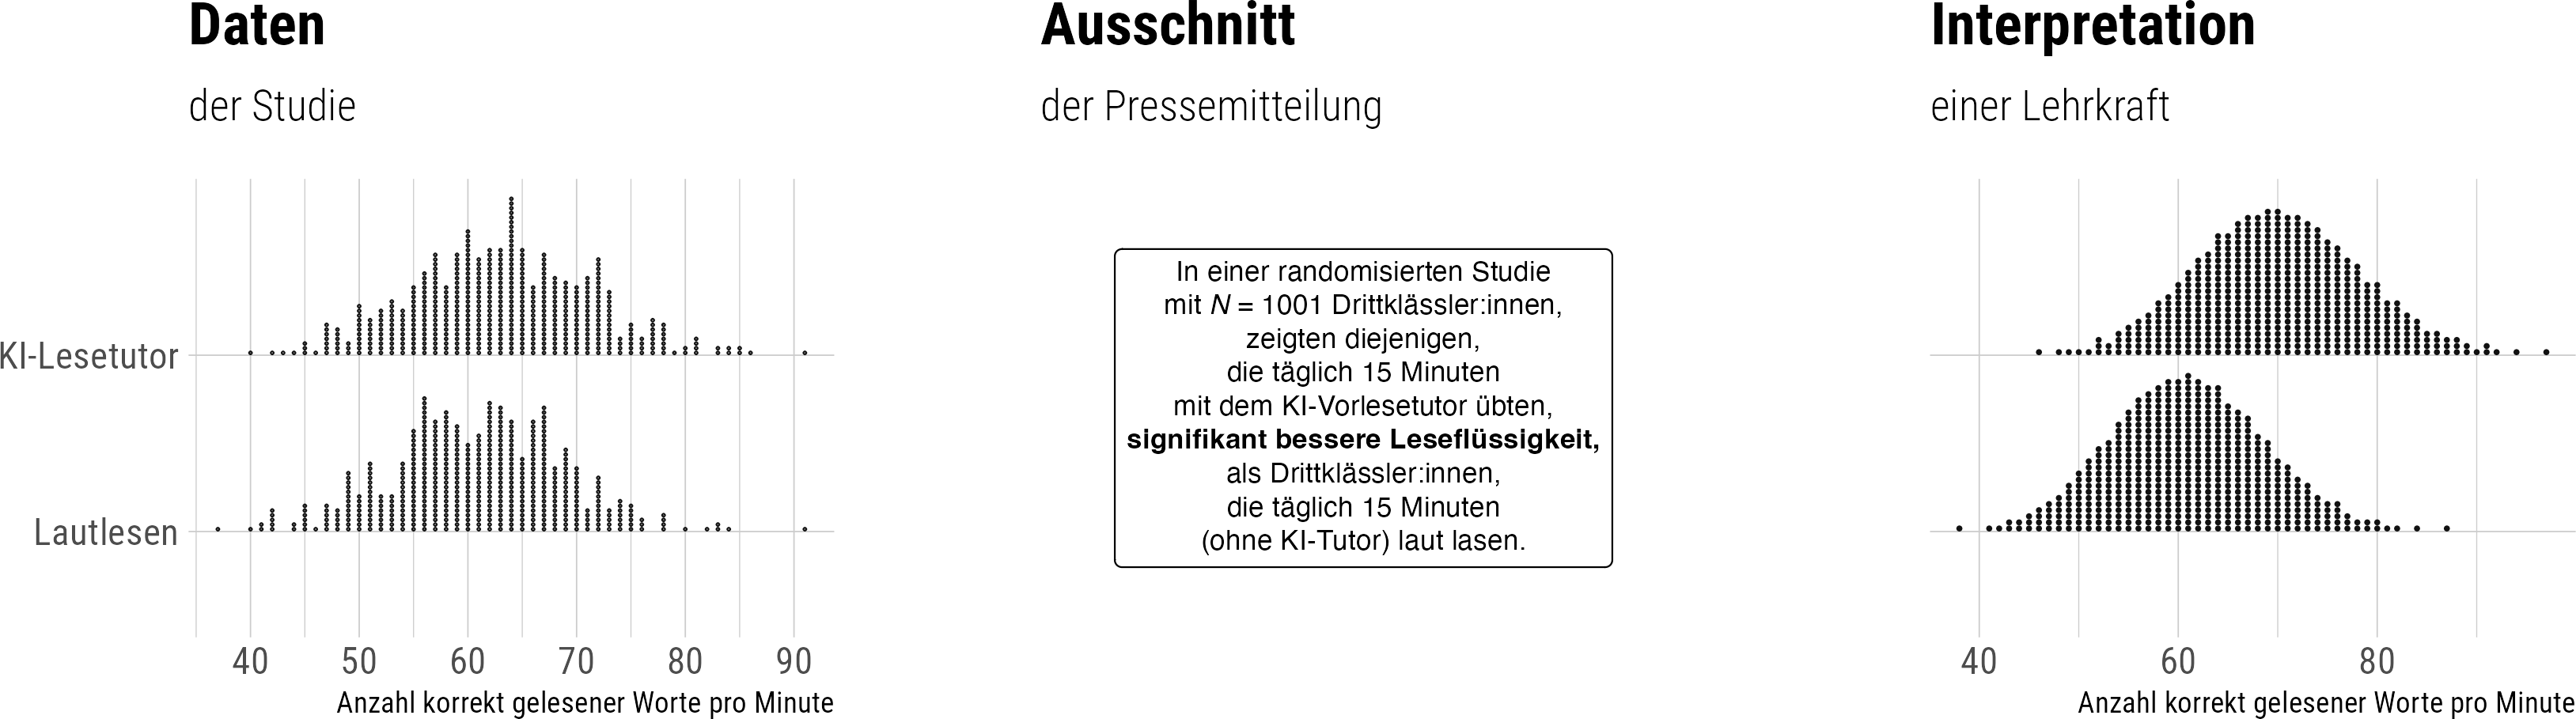
\includegraphics[keepaspectratio]{index_files/figure-pdf/fig-AbbildungMoMa-1.png}}

\end{figure*}

\textsubscript{Quelle:
\href{https://sammerk.github.io/StudienergebnisseBesserKommunizieren/index.qmd.html}{Artikel-Notizbuch}}

Liest eine Lehrkraft etwa die (fiktive) Pressemitteilung in
Abbildung~\ref{fig-AbbildungMoMa}, stellt sich die Ergebnisse darauf
basierend wie in Abbildung~\ref{fig-AbbildungMoMa} rechts vor
(\citeproc{ref-schmidt2023}{Schmidt et al. 2023}) und überzeugt
anschließend ihre Schulleitung, diesen KI-Lesetutor zu beschaffen und
schulweit einzusetzen, liegt höchstwahrscheinlich dysfunktionales
evidenzinformiertes Handeln vor. Während die Forscher:innen mit
»signifikant bessere Leseflüssigkeit« zum Ausdruck bringen, dass ihre
Daten unter der Annahme eines Nulleffekts unwahrscheinlich sind
(signifikanter \emph{p}-Wert), interpretiert die Lehrkraft diese
Formulierung als »Unterschied bedeutsamer Größe«. Folglich
schlussfolgert sie, dass es Sinn macht Geld und Zeit in Anschaffung und
Implementation des KI-Lesetutors zu investieren, weil sie den
KI-Lesetutor für deutlich lernwirksamer hält als lautes Lesen, obwohl
etwa die Implementation von Lautlesetandems lernwirksamer,
kostengünstiger und weniger zeitaufwändig gewesen wäre.

Die Forschung zur Wissenschaftskommunikation hat eine Reihe solcher
potenziellen Problematiken aufgezeigt: Z.B. das soeben beschriebene
Verwechseln von Inferenzstatistik und Effektstärke
(\citeproc{ref-schmidt2023}{Schmidt et al. 2023}), das automatische
Annehmen starker Effekte, wenn keine Effektstärken berichtet wurden
(Practical Significance Bias, \citeproc{ref-michal2024}{Michal und Shah
2024}), Rückschaufehler (\citeproc{ref-masnick2009}{Masnick und
Zimmerman 2009}) oder die verzerrte Einschätzung der Belastbarkeit von
Befunden (z.B. das Ergebnis einer Laborstudie mit \emph{N} = 56 mit
großem Effekt und daher hoher statistischer Power) durch irrelevante
Zahlen (z.B. Stichprobengröße einer zuvor gelesenen Large-Scale-Studie,
\citeproc{ref-bohrer2025}{Bohrer et al. 2025}).

Gleichzeitig liegt eine Reihe von Befunden vor, die implizieren, dass
verbesserte Kommunikation von Evidenz an Lehrkräfte zu Zwecken
evidenzinformierten Handelns vergleichsweise einfach umsetzbar ist (z.B.
\citeproc{ref-schneider2024}{Schneider et al. 2024}). Grundsätzlich
lassen sich die bisherigen Befunde in angebotsseitige und
nutzendenseitige Ansätze unterscheiden, also in Interventionen, die die
Auswahl und Darstellung der Evidenz optimieren möchten und Ansätze, die
bei der Scientific, Data und Statistical Literacy der Lehrkräfte
ansetzen (\citeproc{ref-bruhwiler2020}{Brühwiler und Leutwyler 2020}).

Zu zweiterem gehören Programme wie »Data Teams«
(\citeproc{ref-Schildkamp2018}{Schildkamp et al. 2018}), welche durch
ein umfängliches Set an vordefinierten Leitlinien und Aktivitäten
versucht, konkrete schulische Probleme mit Hilfe von (oft eigens dafür
genierten) Daten zu lösen, wobei meist 4-6 Lehrkräfte und
Schulleiter:innen mit Bildungswissenschaftler:innen und
Fachdidaktiker:innen kooperieren. Hierzu gehören auch
»Brokering-Ansätze« (teilweise auch als »research practice partnerships«
bezeichnet), in welchen Wissenschaftler:innen und Lehrpersonen
(insbesondere Schulleitungen) gemeinsam versuchen, konkrete schulischen
Probleme unter Rückgriff auf wissenschaftliche Erkenntnisse zu lösen
(z.B. \citeproc{ref-sharples2015}{Sharples und Sheard 2015}). Auch Kurz-
(\citeproc{ref-merk2020}{Merk et al. 2020}) oder längerfristig angelegte
(\citeproc{ref-karst2024}{Karst et al. 2024}) Interventionen zur
Anbahnung notwendiger Kompetenzen für evidenzinformiertes Handeln wie
die Interpretation von grafisch dargestellten Daten
(\citeproc{ref-friel2001}{Friel et al. 2001}) oder Forschungskompetenz
(\citeproc{ref-neuenschwander2005}{Neuenschwander 2005}) sowie die
konkrete Unterstützung für evidenzinformiertes Handeln
(\citeproc{ref-zotero-8935}{Clearing House Unterricht Academy 2025}),
können diesem Ansatz zugerechnet werden.

Angebotsseitige Versuche die Kommunikation von Evidenz zu verbessern,
stammen aus verschiedensten Disziplinen: So wird z.B. in der Psychologie
untersucht (\citeproc{ref-grice2020}{Grice et al. 2020}), welche
algebraisch äquivalenten Formulierungen zu standardisierten
Effektstärken bei Rezeption durch Laien adäquatere Vorstellungen
induzieren (siehe Tabelle~\ref{tbl-wisskommbsp}). In der
Human-Computer-Interaction-Forschung werden (teils dynamische)
Visualisierungstechniken entwickelt, um Effektstärken und Inferential
Uncertainty besser zu kommunizieren (z.B.
\citeproc{ref-hullman2015}{Hullman et al. 2015};
\citeproc{ref-zhang2023}{Zhang et al. 2023}). Die
bildungswissenschaftliche Lehrerbildungsforschung sowie die
Fachdidaktiken erproben innovative Formate für die Zielgruppe der
Lehrkräfte (z.B. \citeproc{ref-schneider2024}{Schneider et al. 2024}),
was auch das Anliegen der vorliegenden Studie ist.

\begin{ThreePartTable}

\begin{table}

\caption{\label{tbl-wisskommbsp}Beispiele für angebotsseitige Versuche
verbesserter Kommunikation von Evidenz}

\centering{

\fontsize{9.0pt}{10.8pt}\selectfont
\begin{tabular*}{\linewidth}{@{\extracolsep{\fill}}lll}
\toprule
 & Unterschied & Zusammenhang \\ 
\midrule\addlinespace[2.5pt]
Standard-kommunikation & Die Leseleistung von Schülerinnen und Schülern sank in PISA 2022 um 28 Punkte und damit auf den Tiefststand. & Der sozioökonomische Status klärt 14\% der Varianz der Mathematikleistung auf. \\ 
Verbesserte Kommunikation & Die Leseleistungen von Schülerinnen und Schülern in Deutschland aus PISA 2018 und aus PISA 2022 überlappen sich zu 88,9\%, wobei der Mittelwert um 28 Punkte sank. & Von 100 Schülerinnen und Schülern, die einen überdurchschnittlichen sozioökonomischen Status haben, zeigen 69 eine überdurchschnittliche Mathematikleistung. \\ 
\bottomrule
\end{tabular*}

}

\end{table}%

\end{ThreePartTable}

\textsubscript{Quelle:
\href{https://sammerk.github.io/StudienergebnisseBesserKommunizieren/index.qmd.html}{Artikel-Notizbuch}}

\section{Die vorliegende Studie}\label{die-vorliegende-studie}

In diesem Kontext untersucht die vorliegende Studie, inwiefern
verbreitete Standardgrafiken zur Kommunikation der Entwicklung der
Lesekompetenz in den deutschen Kohorten des Programme of International
Student Assessment (PISA) Practical Significance Bias induzieren und ob
dieser mit Grafiken verringert werden kann, bei deren Gestaltung
theoretische und empirische Erkenntnisse der Wissenschaftkommunikation
(siehe Kapitel~\ref{sec-materialien}) berücksichtigt wurden.

\subsection{Methode}\label{methode}

\subsubsection{Materialien}\label{sec-materialien}

In der wissenschaftlichen wie journalistischen Berichterstattung zu den
Ergebnissen der PISA-2022-Kohorte wurden zahlreiche Darstellungsformate
gewählt, insbesondere Liniendiagramme (siehe
Tabelle~\ref{tbl-pisalinegraphs}), was angesichts der Anlage des PISA
als Trendstudie (\citeproc{ref-duxf6ring2016}{Döring und Bortz 2016})
konsequent erscheint.

\begin{ThreePartTable}

\begin{longtable}[]{@{}
  >{\raggedright\arraybackslash}p{(\linewidth - 4\tabcolsep) * \real{0.3333}}
  >{\raggedright\arraybackslash}p{(\linewidth - 4\tabcolsep) * \real{0.3333}}
  >{\raggedright\arraybackslash}p{(\linewidth - 4\tabcolsep) * \real{0.3333}}@{}}
\caption{Verwendete Liniendiagramme in der
Berichterstattung.}\label{tbl-pisalinegraphs}\tabularnewline
\toprule\noalign{}
\endfirsthead
\endhead
\bottomrule\noalign{}
\endlastfoot
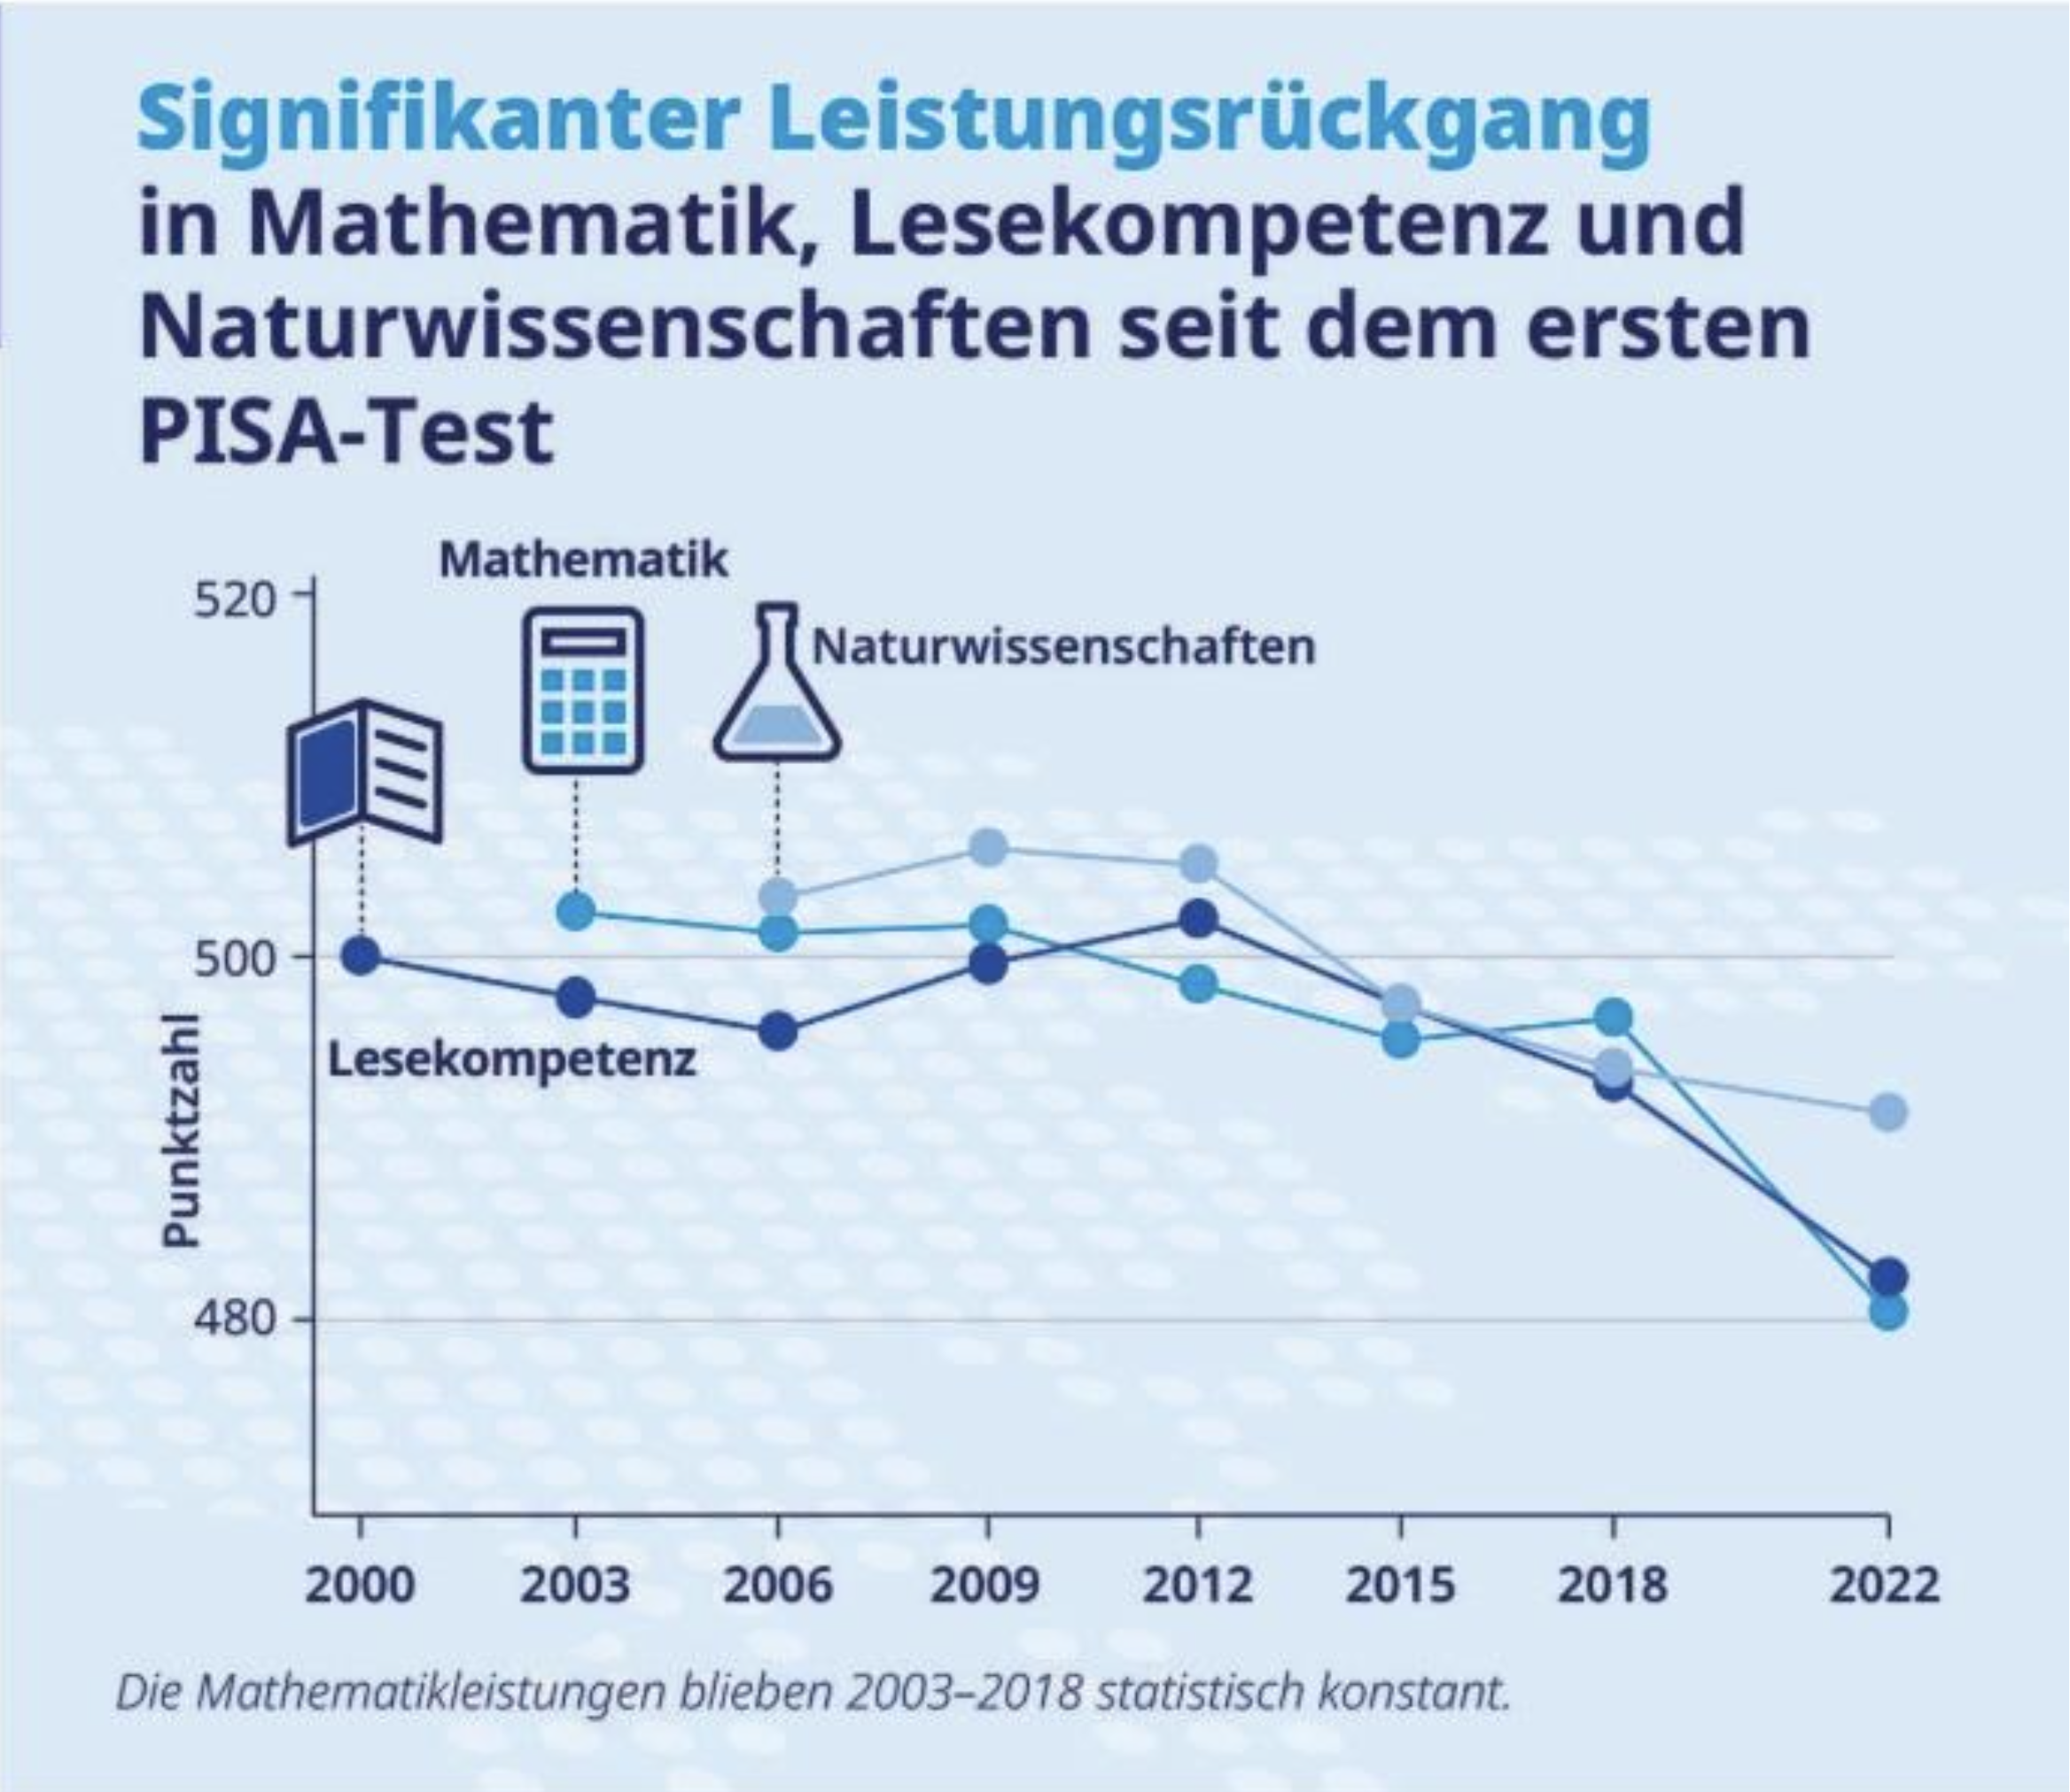
\includegraphics[width=9.375in,height=\textheight,keepaspectratio]{img/oecd.png}
&
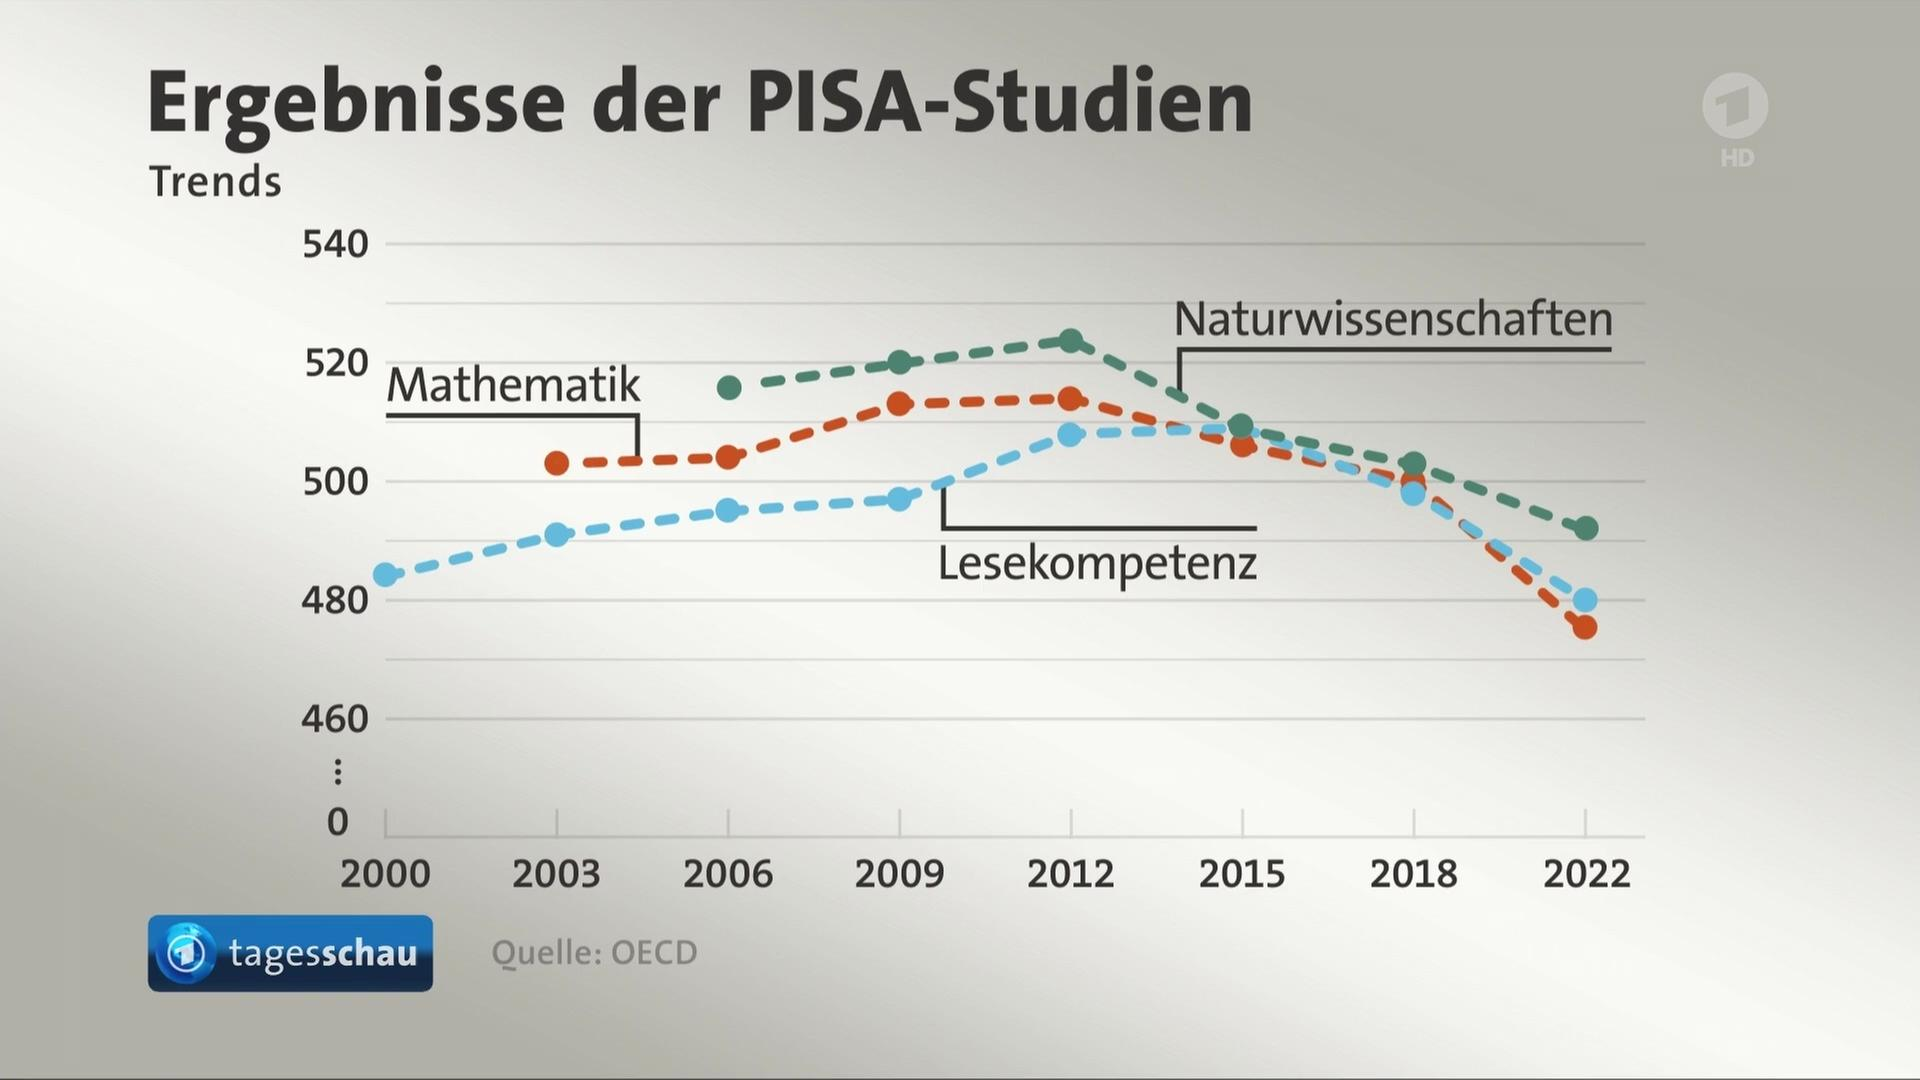
\includegraphics[width=9.375in,height=\textheight,keepaspectratio]{img/tagessschau.jpg}
&
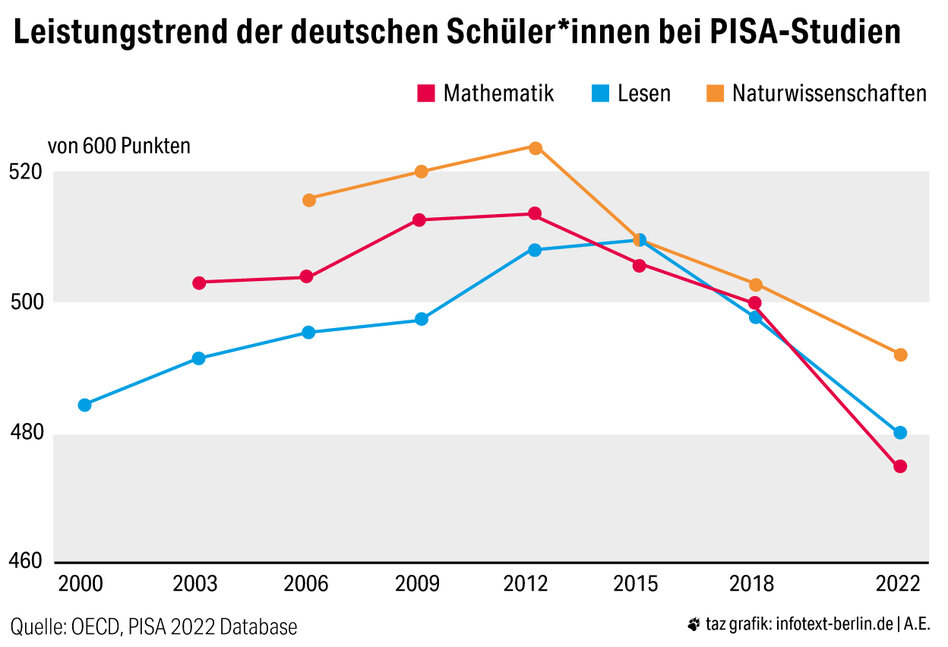
\includegraphics[width=8.33333in,height=\textheight,keepaspectratio]{img/taz.jpeg} \\
OECD (\citeproc{ref-oecd2023a}{2023}) & RBB
(\citeproc{ref-rbb2023}{2023}) & taz
(\citeproc{ref-taz.de2023}{2023}) \\
\end{longtable}

\end{ThreePartTable}

Diese Abbildungen erlauben einen effizienten Vergleich der Mittelwerte
sowohl über die Zeit als auch Variablen (hier: Fächer) hinweg. In
solchen Grafiken ist jedoch die Bedeutsamkeit der Mittelwertsdifferenz
nur bei bekannter Streuung interpretierbar:
Abbildung~\ref{fig-mwdiffstreuung} zeigt jeweils die gleichen
Mittelwerte von 508 (PISA Lesen 2015) und 480 (PISA Lesen 2022).

\phantomsection\label{cell-fig-mwdiffstreuung}
\begin{figure*}[H]

{\caption{{Illustration der Unabhängigkeit von Mittelwertsdifferenz und
Größe des Effekts}{\label{fig-mwdiffstreuung}}}}

\pandocbounded{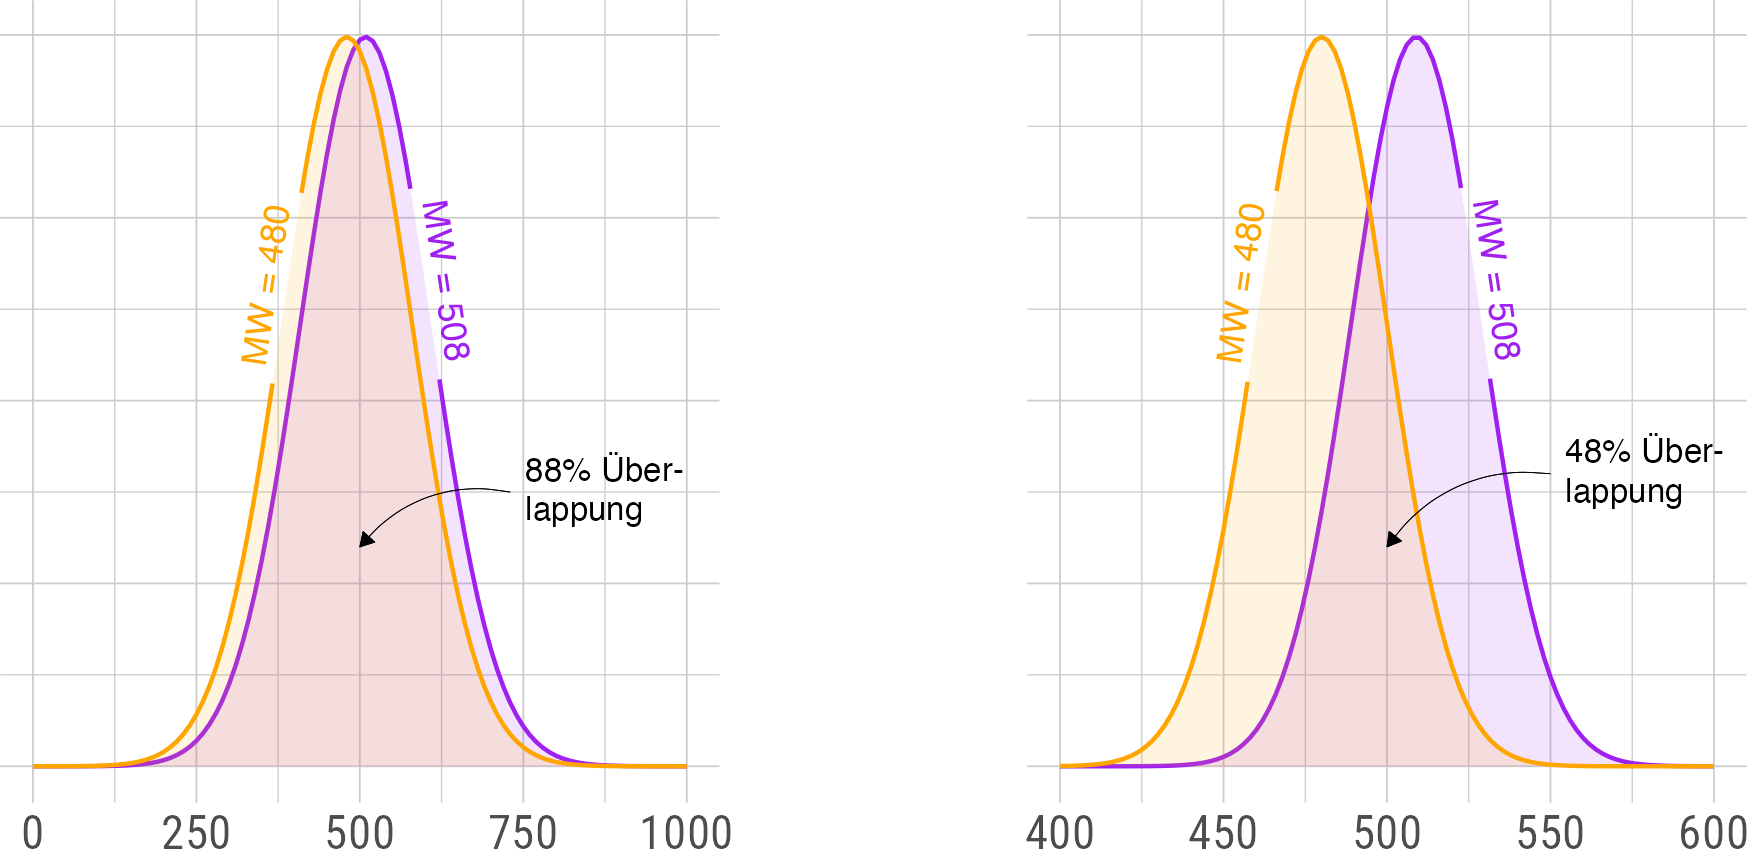
\includegraphics[keepaspectratio]{index_files/figure-pdf/fig-mwdiffstreuung-1.png}}

\end{figure*}

\textsubscript{Quelle:
\href{https://sammerk.github.io/StudienergebnisseBesserKommunizieren/index.qmd.html}{Artikel-Notizbuch}}

Das Ausmaß der Bedeutsamkeit dieses (gleichen) Mittelwertsunterschiedes
entsteht aber erst durch die Streuung der Daten um diesen Mittelwert
herum. Weil die Variablen im rechten Teil der Abbildung weniger streuen,
ist die Überlappung der beiden Gruppen geringer (48\%, großer Effekt),
während die große Überlappung im linken Teil (88\%, kleiner Effekt)
durch die große Streuung zustande kommt. Die Abbildungen in
Tabelle~\ref{tbl-pisalinegraphs} sagen also nicht nur nichts über die
Bedeutsamkeit der Mittelwertsunterschiede aus. Die nicht dargestellte
Varianz induziert möglicherweise auch eine wahrgenommene große
Bedeutsamkeit der Mittelwertsdifferenz (\citeproc{ref-kale2021}{Kale et
al. 2021}).

\begin{ThreePartTable}

\begin{longtable}[]{@{}
  >{\raggedright\arraybackslash}p{(\linewidth - 2\tabcolsep) * \real{0.4444}}
  >{\raggedright\arraybackslash}p{(\linewidth - 2\tabcolsep) * \real{0.5556}}@{}}
\caption{Verwendete Stimuli}\label{tbl-materials}\tabularnewline
\toprule\noalign{}
\endfirsthead
\endhead
\bottomrule\noalign{}
\endlastfoot
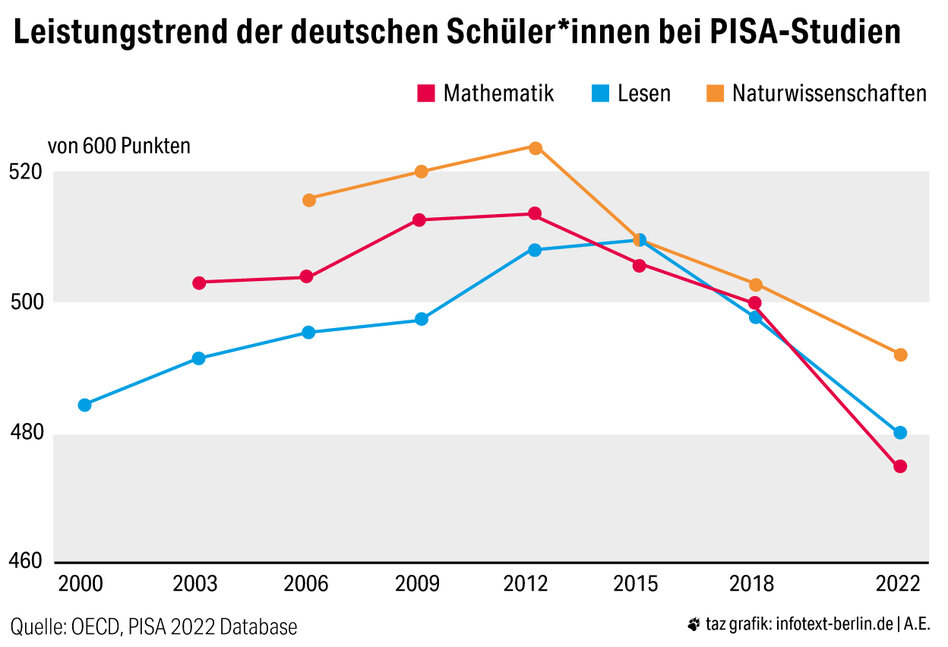
\includegraphics[width=4.16667in,height=\textheight,keepaspectratio]{img/taz.jpeg}
&
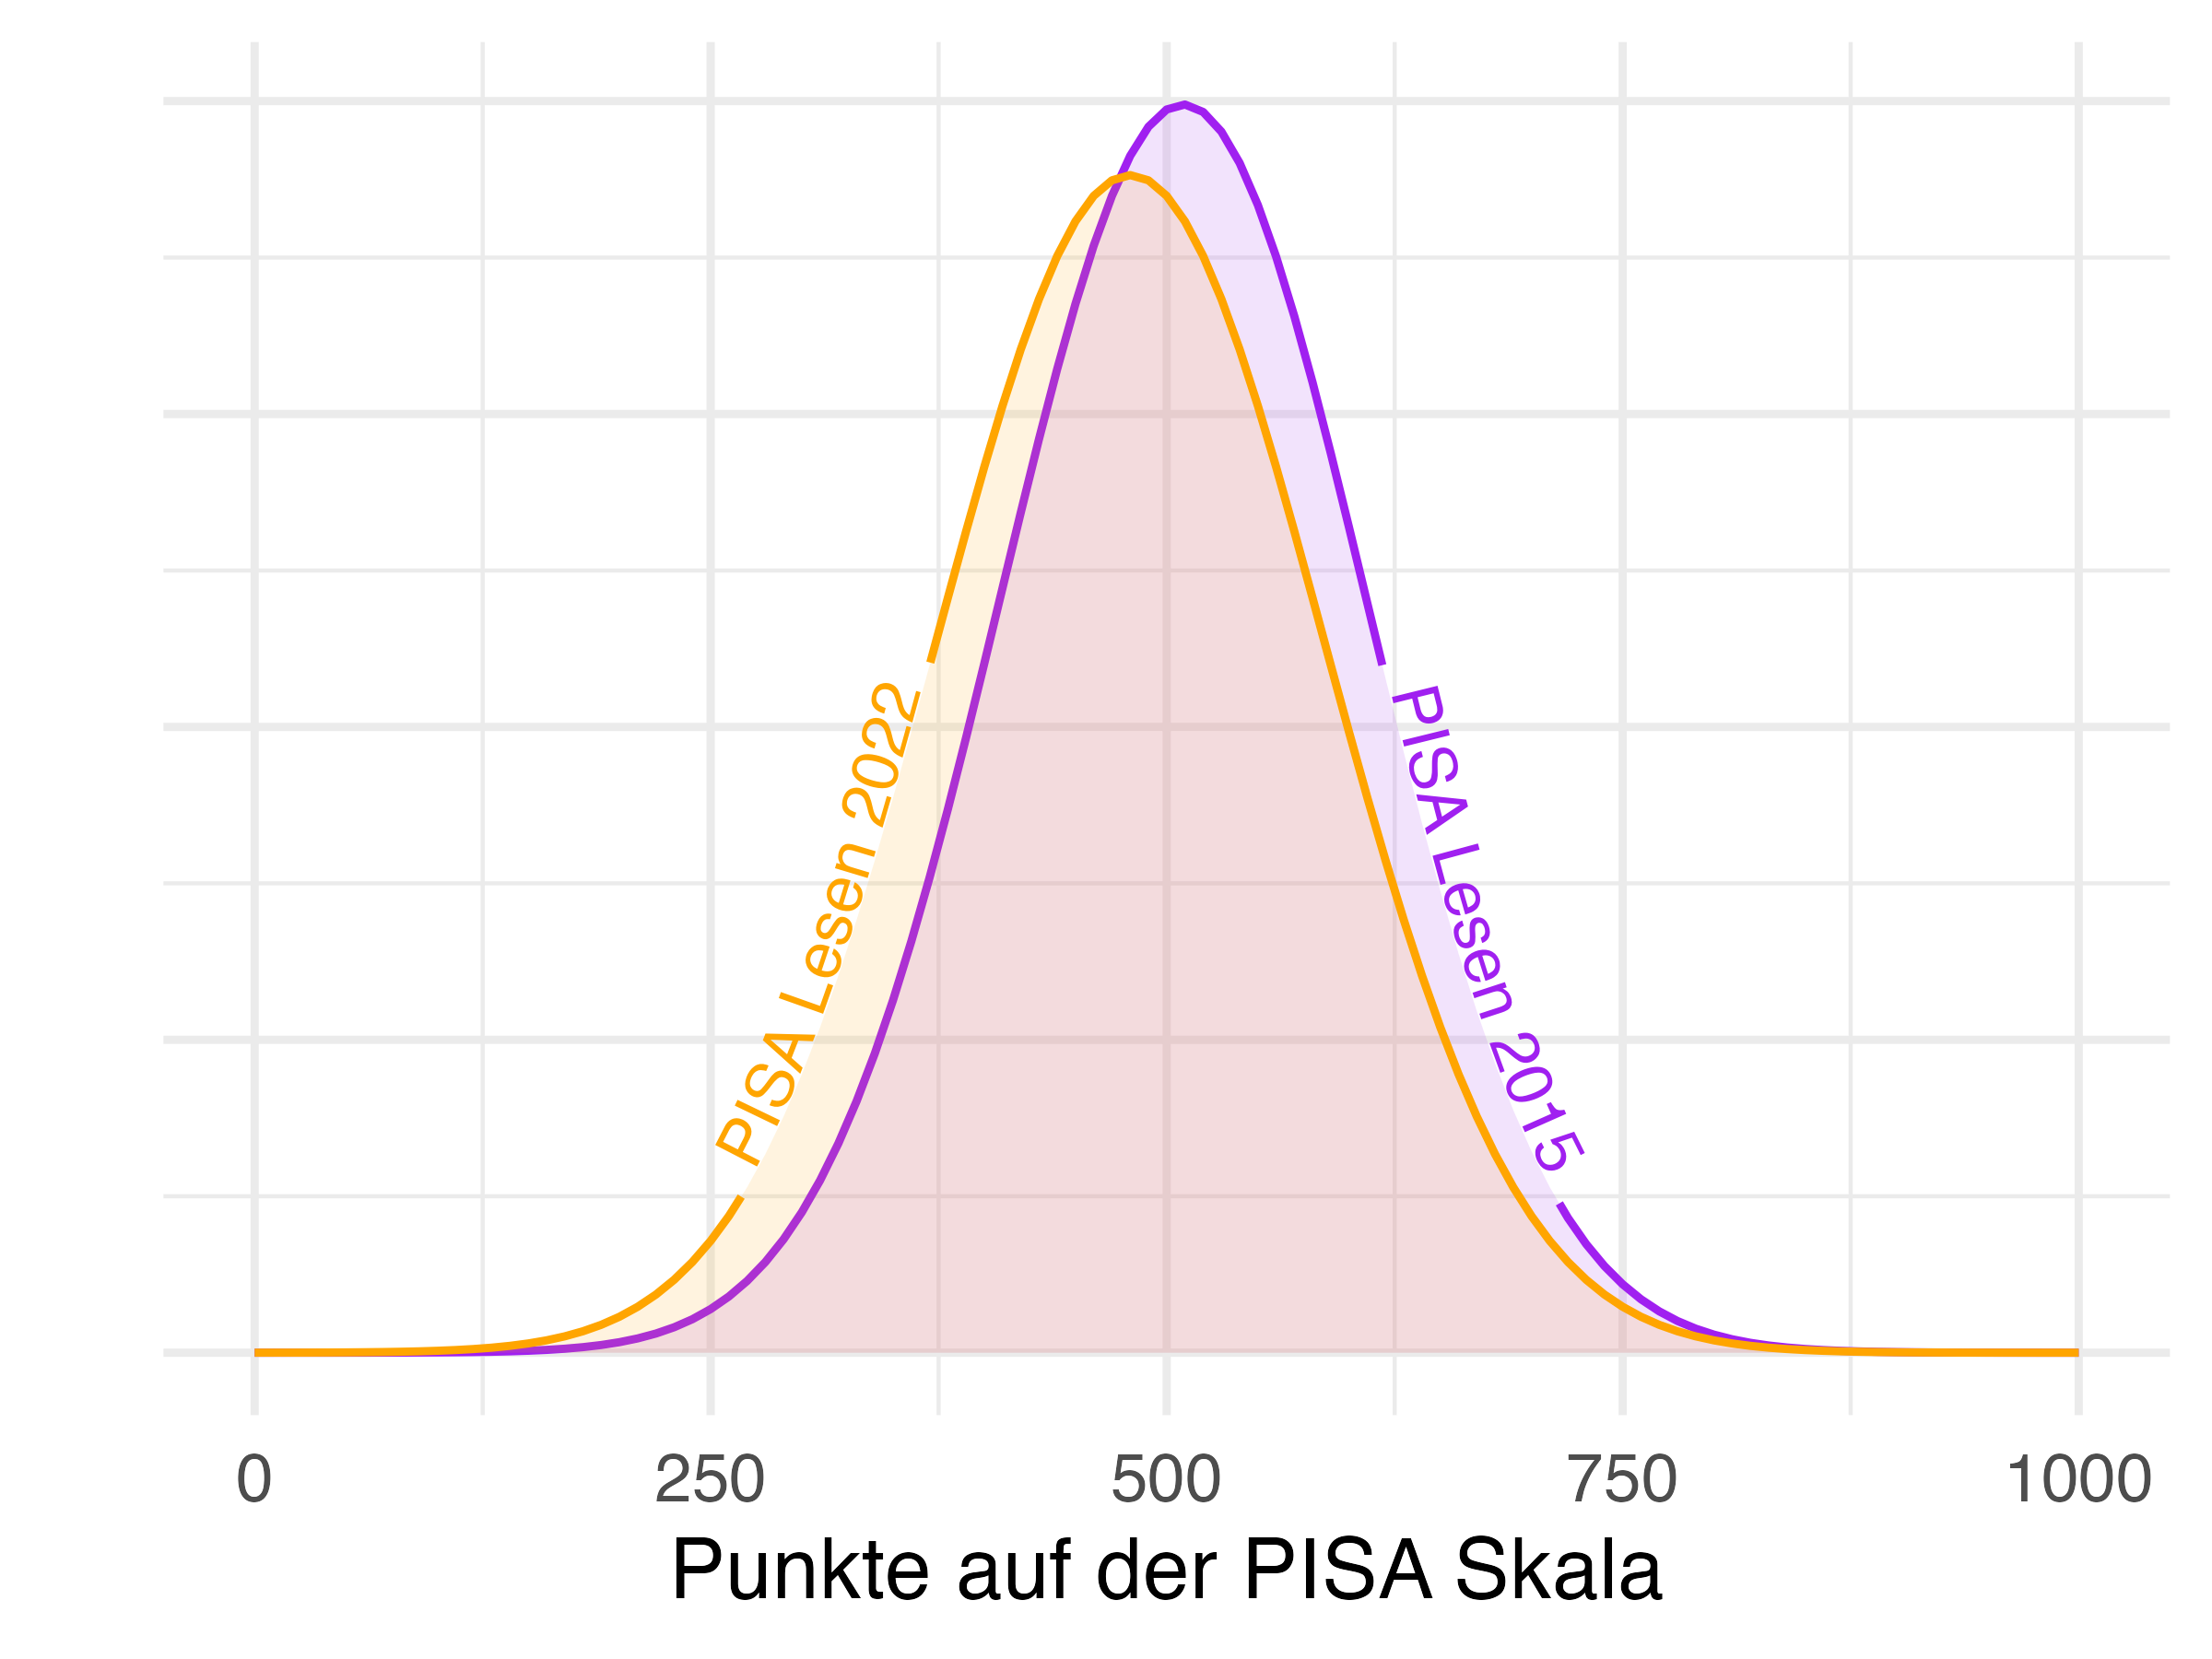
\includegraphics[width=3.78125in,height=\textheight,keepaspectratio]{img/geomtextline.png} \\
\end{longtable}

\end{ThreePartTable}

Daher wurden vorliegend neben Liniendiagrammen auch überlappende
Verteilungskurven verwendet. Um diese barriereärmer zu gestalten wurde
bei der Farbgebung auf hinreichenden Kontrast bei den prävalenten
Sehbehinderungen geachtet (\citeproc{ref-garnier2023}{Garnier et al.
2023}). Um unnötige Arbeitsgedächtnisbelastung zu vermeiden, wurde die
Legende direkt in die Grafik integriert
(\citeproc{ref-franconeri2021}{Franconeri et al. 2021}).

\subsubsection{Design, Stichprobe und
Instrument}\label{design-stichprobe-und-instrument}

\textsubscript{Quelle:
\href{https://sammerk.github.io/StudienergebnisseBesserKommunizieren/index.qmd.html}{Artikel-Notizbuch}}

In einem Between-Person Design wurde \emph{N} = 195 Studierenden in
Bachelorstudiengängen des Primar- und Sekundarstufenlehramtes
randomisiert eine der beiden in Tabelle~\ref{tbl-materials}
dargestellten Abbildungen gezeigt. Anschließend wurden sie mit folgenden
Stimulus aufgefordert, die Effektstärke einzuschätzen: ``\emph{Basierend
auf dieser Grafik: Wie hoch schätzen (exakte Antwort nicht möglich) Sie
die Wahrscheinlichkeit ein, dass eine zufällig gezogene Schülerin oder
ein zufällig gezogener Schüler aus dem Jahr 2022 im Lesen schlechter
abschneidet als eine zufällig gezogene Schülerin oder Schüler aus dem
Jahr 2015}?''. Beantwortet wurde diese Frage mit einem Schieberegler,
dessen Enden mit ``\emph{50\% (beide Gruppen gleich)}'' und
``\emph{100\%} \emph{(maximaler Effekt)}'' beschriftet waren. Diese
Erfassung der wahrgenommenen Effektstärke als »Probability of
Superiority« ist in der Human-Computer-Interaction-Forschung verbreitet
und gilt als valide (\citeproc{ref-brooks2014}{Brooks et al. 2014};
\citeproc{ref-kim2022}{Kim et al. 2022}), wenngleich die
Operationalisierung als Schieberegeler unklar lässt, inwiefern bei der
Beantwortung tatsächlich eine Elaboration der Überlappung vorgenommen
wird oder die Teilnehmenden eher intutiv (etwa wie bei einem
Likert-Item) vorgehen.

\subsubsection{Statistische Analyse}\label{statistische-analyse}

Die abhängige Variable »Wahrgenommene Effektstärke« (operationalisiert
als Probability of Superiority) ist per Design auf das geschlossene
Intervall {[}0,5; 1{]} beschränkt und zeigt empirisch Bimodalität (siehe
Abbildung~\ref{fig-plotresults}). Um diesen Umständen in der
inferenzstatistischen Modellierung Rechnung zu tragen, wurden
bayesianische Mixture Regressionsmodelle für zwei trunkierte
Normalverteilungen (\citeproc{ref-frischkorn2023}{Frischkorn und Popov
2023}) in der probabilistischen Sprache Stan
(\citeproc{ref-standevelopmentteam2024}{Stan Development Team 2024})
mithilfe des R-Pakets \{brms\} (\citeproc{ref-buxfcrkner2017}{Bürkner
2017}) geschätzt.

\textsubscript{Quelle:
\href{https://sammerk.github.io/StudienergebnisseBesserKommunizieren/index.qmd.html}{Artikel-Notizbuch}}

\subsubsection{Ergebnisse}\label{ergebnisse}

Die Inspektion des Marcov-Chain-Monte-Carlo-Sampling-Prozesses zeigte
eine zufriedenstellende Qualität bzgl. Konvergenz \((\hat{R} < 1.01)\)
und effektiver Sampling Size (\(ESS_{Bulk} > 1000 < ESS_{Tail}\),
\citeproc{ref-vehtari2021prefix}{Vehtari et al. 2021}).

\phantomsection\label{cell-fig-plotresults}
\begin{figure*}[H]

{\caption{{Geschätze Effektstärke (Probability of Superiority) nach
Stimulus. Beide Gruppen zeigen einen sehr deutlichen Practical
Significance Bias (Abstand von Median und wahrem
Wert).}{\label{fig-plotresults}}}}

\pandocbounded{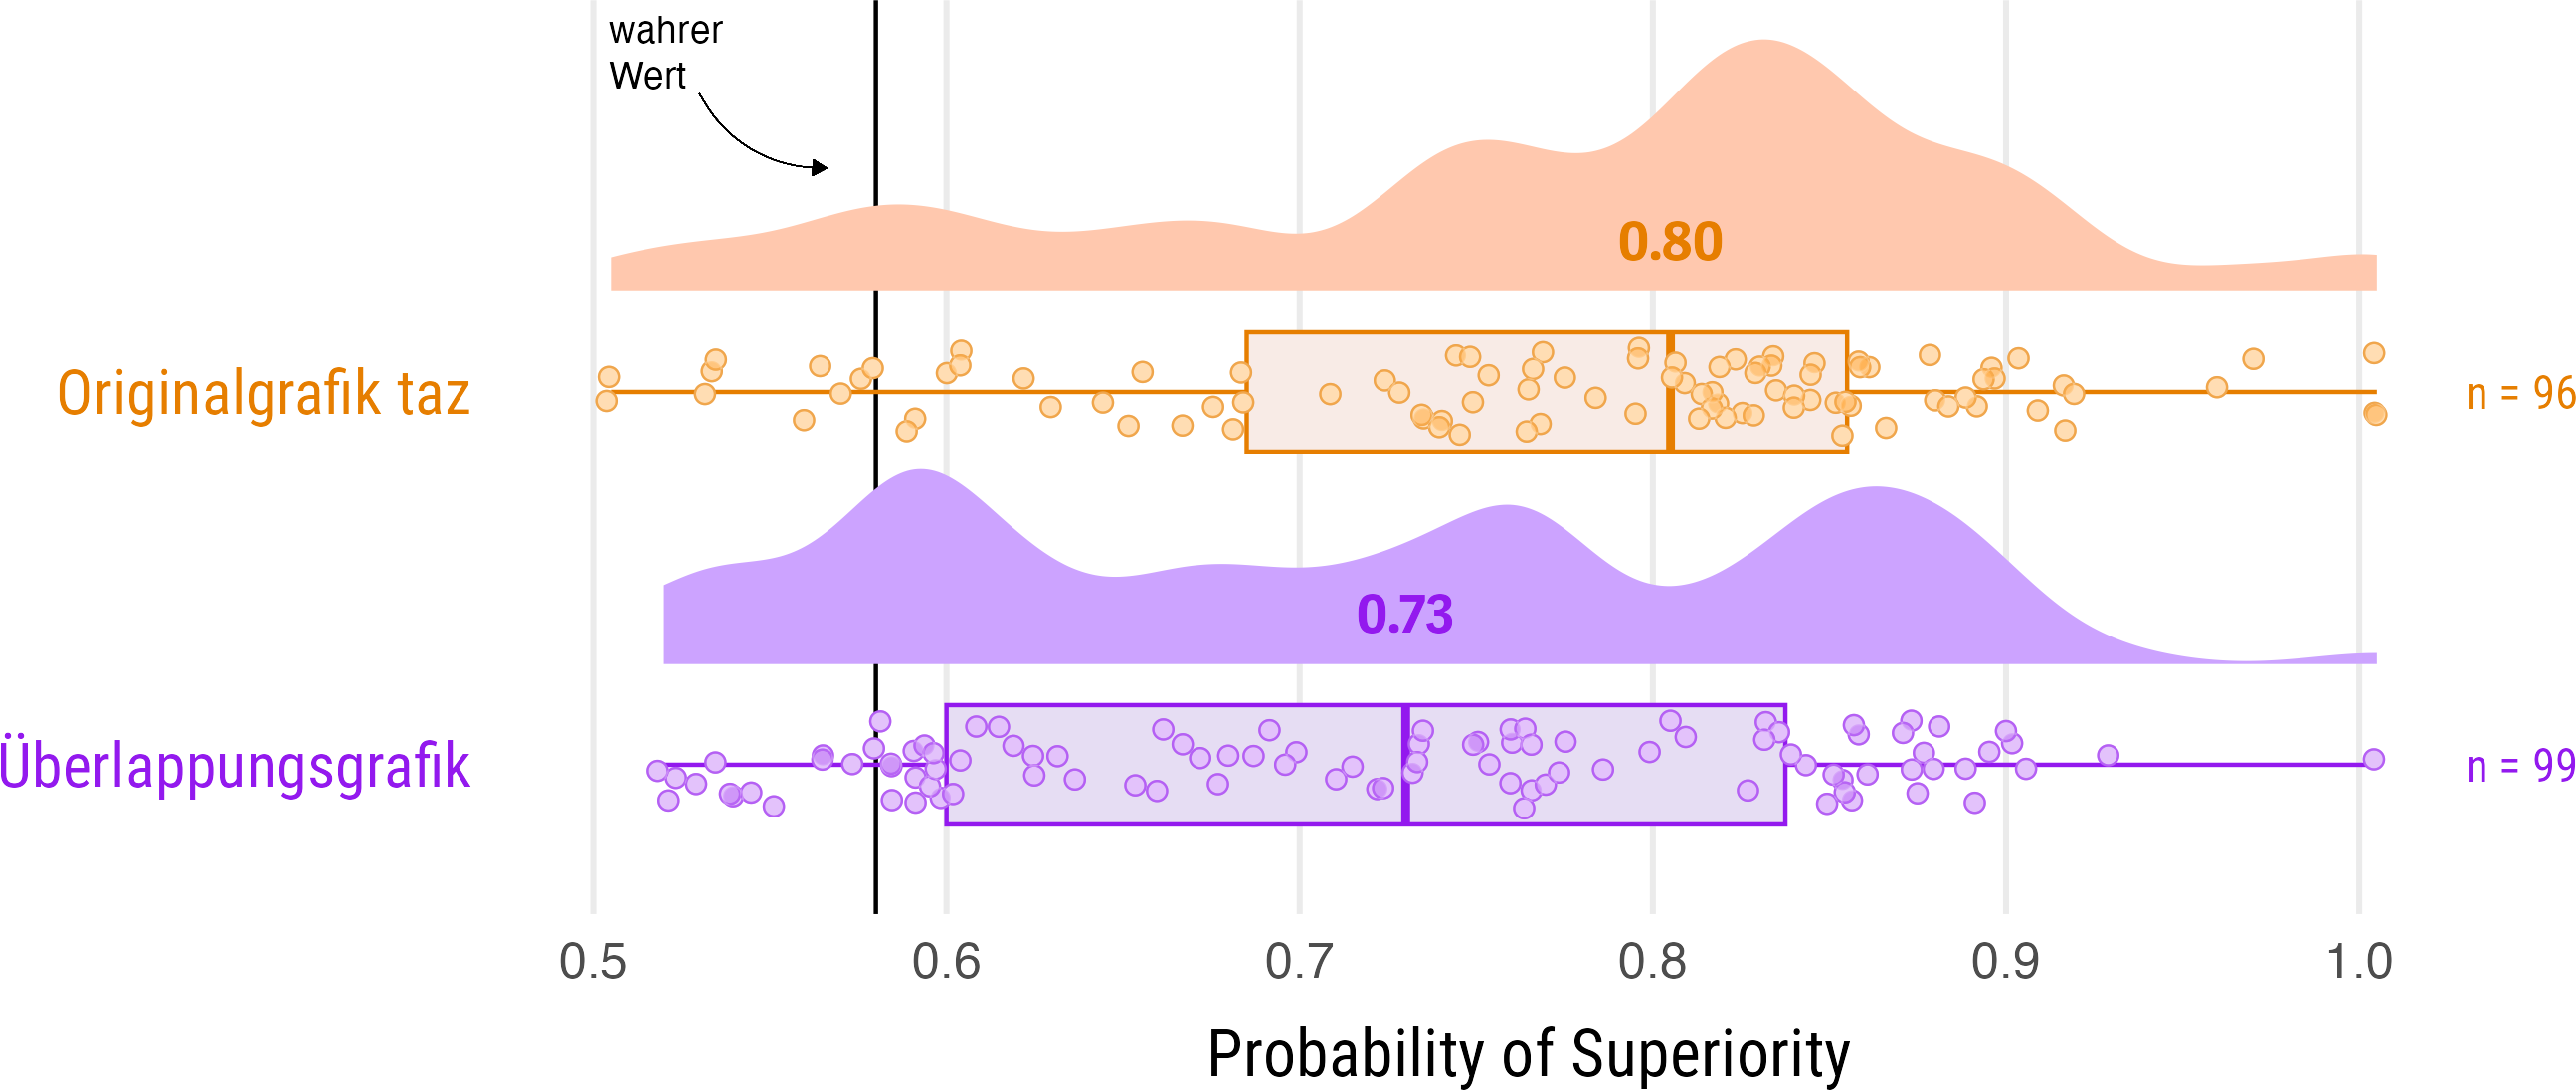
\includegraphics[keepaspectratio]{index_files/figure-pdf/fig-plotresults-1.png}}

\end{figure*}

\textsubscript{Quelle:
\href{https://sammerk.github.io/StudienergebnisseBesserKommunizieren/index.qmd.html}{Artikel-Notizbuch}}

Die Medianeinschätzung der Probability of Superiority lag in beiden
Gruppen deutlich über dem wahren Wert (Liniendiagramm .80, überlappende
Überlappungsgrafik .73). Dieser Unterschied in der Einschätzung
entspricht einer Überlappung von 81.71\% (Cliff's \emph{d} = 0.23) oder
anders ausgedrückt: Legt man 100 mal einem:einer Studierenden die
Originalgrafik und einem:einer Studierenden die Überlappungsgrafik vor,
schätzt 61mal die:der Studierende mit der Überlappungsgrafik den Effekt
weniger verzerrt ein. Die Inferenzstatistik für diesen Unterschied ist
mit einer Evidence Ratio von 14.8 klar konklusiv: Die
Alternativhypothese einer kleineren Probability of Superiority für die
Überlappungsgrafik ist gegeben die Daten 14,8-fach wahrscheinlicher als
die Nullhypothese einer größeren Probability of Superiority.

\section{Diskussion}\label{diskussion}

Der vorliegende Beitrag zielt darauf ab, zu eruieren, inwiefern es nach
dem Stand der Forschung gestaltete Wissenschaftskommunikation
ermöglicht, bildungswissenschaftliche und fachdidaktische Evidenz
»besser« an Lehrkräfte zu kommunizieren. Dabei wurde »besser« als
»weniger gebiased« operationalisiert und gezeigt, dass die Wahl einer
theoretisch fundierten grafischen Darstellung einen deutlich geringeren
Bias induzierte als eine Standardgrafik. Allerdings war auch die
Rezeption der verbesserten Darstellung immer noch erheblich verzerrt
(siehe Abbildung~\ref{fig-plotresults}).

Im Lichte dieser Ergebnisse werden im Folgenden drei Implikationen
diskutiert: 1) Die Forderung, dass Lehrkäfte ihre professionelle Praxis
evidenzinformiert gestalten sollen, setzt Anstrengungen in der
Wissenschaftskommunikation seitens Bildungswissenschaften und
Fachdidaktiken voraus. 2) Inwiefern diese Anstrengungen zielführend
sind, sollte empirisch überprüft werden. 3) Erfolgreiche
Wissenschaftskommunikation in den Bildungswissenschaften und
Fachdidaktiken impliziert eine Passung von Angebots- und
Nutzendenmerkmalen und damit einen dialogischen Prozess für die
Entwicklung einer solchen Passung.

Sowohl Wissenschaftstheorie (z.B. \citeproc{ref-mitchell2010}{Mitchell
und Jolley 2010}) als auch bildungswissenschaftliche Literatur (z.B.
\citeproc{ref-bohl2015a}{Bohl et al. 2015}; \citeproc{ref-dewe1992}{Dewe
et al. 1992}) haben die Möglichkeiten und Limitationen der
Abgrenzbarkeit von »Wissenschaft« und »Nicht-Wissenschaft« (bzw. in den
Bildungswissenschaften von »Theorie« und »Praxis«) diskutiert und heben
u.a. hervor, dass Entitäten und Aussagen in ihrer Bedeutung primär an
den Herkunftskontext (z.B. »Wissenschaft« oder »Praxis«) gebunden sind.
Also ist auch z.B. die »Evidenz« einer explanativen
bildungswissenschaftlichen Studie per se zunächst
bildungswissenschaftlich und muss für eine evidenzinformierte Handlung
in der Praxis reinterpretiert werden (z.B.
\citeproc{ref-grouxdfophoff2023}{Groß Ophoff et al. 2023}). Damit liegt
es auf der Hand, dass sich Bildungswissenschaftler:innen und
Fachdidaktiker:innen fragen sollten, welche
»wissenschaftlichen/theoretischen« Entitäten (z.B. Effektstärken oder
inferenzstatistischen Maße) und Aussagen (z.B. kausale Effekte) sie wie
in die Kommunikation ihrer Ergebnisse gegenüber der Praxis aufnehmen.

Dass diese Forderung selbst rein innerwissenschaftlich betrachtet nicht
trivial ist, zeigt z.B. die Tatsache, dass Guidelines von
Fachgesellschaften wie z.B. der American Psychological Association
(\citeproc{ref-americanpsychologicalassociation2019}{2019}) die
Verwendung von Effektstärken fordern, diese aber in Pressemitteilungen
(etwa der American Educational Research Association) und selbst in
Fachzeitschriften selten sind, obwohl die Fachgesellschaften bzw.
Zeitschriften diese in ihren Autor:innenrichtlinien verbindlich fordern
(\citeproc{ref-mcmillan2011}{McMillan und Jennifer 2011}). Für eine
Wissenschaftskommunikation, die sich an die Praxis richtet scheint es
also plausibel, zu schlussfolgern, dass es unter Forschenden noch nicht
verbreitet scheint, sich literaturbasiert darüber Gedanken zu machen,
inwiefern die eigene Wissenschaftskommunikation z.B. für Lehrkräfte
günstig rezipierbar ist.

Doch selbst ein Bewusstsein für die Fallstricke der Kommunikation
wissenschaftlicher Ergebnisse schützt nicht zwangläufig vor der
Induktion von Fehlvorstellungen: So fanden Schneider et al.
(\citeproc{ref-schneider2024}{2024}) etwa, dass selbst eine als leicht
verständlich geltende Effektstärke für Mittelwertsvergleiche (wie etwa
Cohen's \(U_3\)) bei einem erheblichen Anteil (≥ 29\%) der
Rezipient:innen zu Fehlvorstellungen führte. Die erste Implikation,
scheint also nicht hinreichend für eine gelingende Kommunikation von
Evidenz an Lehrkräfte. Dies führt zur zweiten Implikation: Forschende
sollten nicht nur den Stand der Forschung bei der Kommunikation von
Evidenz berücksichtigen, sondern auch in intern und extern validen
Studien untersuchen, inwieweit diese Berücksichtigung erfolgreich war.
Denn statistische Informationen werden nicht nur von unterschiedlichen
Berufsgruppen (\citeproc{ref-mcdowell2017}{McDowell und Jacobs 2017}),
sondern auch in unterschiedlichen geografischen Regionen differentiell
interpretiert (\citeproc{ref-gigerenzer2005}{Gigerenzer et al. 2005}).
Inwiefern sich also generische Determinaten erfolgreicher
Wissenschaftskommunikation auf die Kommunikation von Evidenz an
Lehrkräfte etwa in einem bestimmten Teil eines Bildungssystems
übertragen lassen, scheint nur schwer a priori bestimmbar.

Was aber, wenn Forschende ihre Wissenschaftskommunikation
literaturbasiert verbessern, aber in empirischen Experimenten sehen,
dass sie dennoch deutlich verzerrt, verrauscht oder konzeptuell falsch
rezipiert wird? Der vorliegende Beitrag macht als dritte Implikation den
Vorschlag, den Kommunikation von Evidenz an Lehrkräfte dialogisch
weiterzuentwickeln und zu berücksichtigen, dass bei der Rezeption von
vermutlich eine komplexe Interaktion von Angebots- und
Nutzendenmerkmalen (\citeproc{ref-bruhwiler2020}{Brühwiler und Leutwyler
2020}) sowie Bottom-Up- bzw. Top-Down-Prozessen
(\citeproc{ref-schmidt2024}{Schmidt 2024}) vorliegt: Man stelle sich
eine Lehrkraft vor, die auf der Suche nach einer Entscheidungsgrundlage
für oder gegen eine unterrichtsgestalterische Maßnahme A auf der Seite
eines Clearing Houses landet. Dort liest sie, dass über viele Studien
gemittelt Maßnahme A dazu geführt hat, dass 63\% der Schülerinnen und
Schüler bessere Leistungen zeigen als der Mittelwert der Schülerinnen
und Schüler mit Maßnahme B. Dann können daraus manche Lehrkräfte
möglicherweise anhand ihres Vorwissens unmittelbar eine
korrekte/konsistente Vorstellung der Effektstärke dieses Unterschieds
\emph{schlussfolgern} (z.B. zwei Normalverteilungen mit 87\%
Überlappung). Hier läge ein Top-Down-Prozess vor, da die Merkmale der
Kommunikation mit den im Langzeitgedächtnis der Rezipient:in vorhandenen
Dispositionen wie Graph, Data oder Statistical Literacy dazu führen,
dass in einem Schlussfolgerungsprozess ein korrektes mentales Modell
erstellt wird. Umgekehrt kann es passieren, dass eine Lehrkraft auf
diese Formulierung stößt und eben kein auf Wissen basierendes mentales
Modell abrufen kann - aber sich Stück für Stück mithilfe der gegebenen
Informationen ein konsistentes mentales Modell erarbeitet. Dabei
\emph{lernt} sie, d.h. erwirbt Graph, Data, oder Statistical Literacy,
was einem Bottom-Up Prozess entspricht. Da Lehrkräfte über sehr
unterschiedliche Dispositionen zu Top-Down-Prozessen verfügen, aber auch
Bottom-Up-Prozesse sehr individuell verlaufen dürften, liegt die dritte
Implikation nahe: Die Kommunikation von Evidenz an Lehrkräfte sollte als
dialogischer und differenzieller Prozess aufgefasst werden. Demnach
würden zum einen Bildungswissenschaftler:innen und Fachdidaktiker:innen
Kenntnis über Top-Down- und Bottom-Up-Prozesse ihrer Rezipienten:innen
erwerben und deren Ausprägung und Entwicklung z.B. anhand von
Think-Aloud-Studien wie z.B. Bez et al. (\citeproc{ref-bez2021}{2021})
beobachten und daraufhin ihre Angebote entsprechend differenzieren und
anpassen. Zum anderen könnten Lehrkräfte in die Entwicklung von
Kommunikationsprodukten anhand kokonstruktiver Verfahren eingebunden
werden, in der Hoffnung, dass eine solche Kooperation von Akteuren aus
den Systemen »Wissenschaft/Theorie« und »Nicht-Wissenschaft/Praxis« dazu
führt, dass innerhalb dieser Systeme Ausdrucksweisen verfügbar werden,
die zu verlustfreieren und damit erfolgreicheren Kommunikationsprozessen
führen können (\citeproc{ref-leitz2024}{Leitz et al. 2024}).

\subsection{Literatur}\label{literatur}

\phantomsection\label{refs}
\begin{CSLReferences}{1}{0}
\bibitem[\citeproctext]{ref-aero2023}
AERO. (2023). \emph{Evidence-Based Teaching Practices}. Australian
Education Research Organisation.
\url{https://www.education.gov.au/quality-initial-teacher-education-review/resources/aero-evidence-based-teaching-practices}

\bibitem[\citeproctext]{ref-altrichter2006}
Altrichter, H., \& Rolff, H.-G. (2006). Datenbasierte Schulentwicklung.
Editorial. \emph{Journal für Schulentwicklung}, \emph{10}(4), 4--6.

\bibitem[\citeproctext]{ref-americanpsychologicalassociation2019}
Association, A. P. (2019). \emph{Publication Manual of the American
Psychological Association} (7. Aufl.). American Psychological
Association.

\bibitem[\citeproctext]{ref-bauer2012}
Bauer, J., \& Prenzel, M. (2012). European teacher training reforms.
\emph{Science}, \emph{336}(6089), 1642--1643.
\url{https://doi.org/10.1126/science.1218387}

\bibitem[\citeproctext]{ref-bauer1978}
Bauer, K.-O., \& Rolff, H.-G. (1978). Vorarbeiten zu einer Theorie der
Schulentwicklung. In K.-O. Bauer \& H.-G. Rolff (Hrsg.), (S. 219--263).
Weinheim und Basel: Beltz.

\bibitem[\citeproctext]{ref-bez2021}
Bez, S., Poindl, S., Bohl, T., \& Merk, S. (2021). Wie werden
Rückmeldungen von Vergleichsarbeiten rezipiert? \emph{Zeitschrift für
Pädagogik}, \emph{67}(4), 551--572.
\url{https://doi.org/10.3262/ZP2104551}

\bibitem[\citeproctext]{ref-bohl2020}
Bohl, T. (2020). Theorien der Schulentwicklung. In M. Harant, P. Thomas,
\& U. Küchler (Hrsg.), (S. 97--109). Tübingen: Tübingen University
Press. \url{https://doi.org/10.15496/publikation-45627}

\bibitem[\citeproctext]{ref-bohl2015a}
Bohl, T., Wacker, A., \& Harant, M. (2015). \emph{Schulpädagogik und
Schultheorie} (1. Aufl.). Stuttgart: UTB GmbH.
\url{https://doi.org/10.36198/9783838541808}

\bibitem[\citeproctext]{ref-bohrer2025}
Bohrer, K., Schmidt, K., \& Merk, S. (2025). Zwei Studien, ein Ergebnis:
Lehramtsstudierende unterliegen im Umgang mit Evidenz dem Ankereffekt.
\emph{Zeitschrift für Erziehungswissenschaft}.

\bibitem[\citeproctext]{ref-bromme2014e}
Bromme, R., Prenzel, M., \& Jäger, M. (2014). Empirische
Bildungsforschung und evidenzbasierte Bildungspolitik. \emph{Zeitschrift
für Erziehungswissenschaft}, \emph{17}(4), 3--54.
\url{https://doi.org/10.1007/s11618-014-0514-5}

\bibitem[\citeproctext]{ref-brooks2014}
Brooks, M. E., Dalal, D. K., \& Nolan, K. P. (2014). Are common language
effect sizes easier to understand than traditional effect sizes?
\emph{Journal of Applied Psychology}, \emph{99}(2), 332--340.
\url{https://doi.org/10.1037/a0034745}

\bibitem[\citeproctext]{ref-bruegelmann2018}
Brügelmann, H. (2018). Unterrichts- und Schulentwicklung in Communities
of Practice. In H. Barz (Hrsg.), (S. 479--484). Wiesbaden: Springer
Fachmedien. \url{https://doi.org/10.1007/978-3-658-07491-3_44}

\bibitem[\citeproctext]{ref-bruhwiler2020}
Brühwiler, C., \& Leutwyler, B. (2020). Praxisrelevanz von Forschung als
gemeinsame Aufgabe von Wissenschaft und Praxis: Entwurf eines
Angebots-Nutzungs-Modells. \emph{BzL - Beiträge zur Lehrerinnen- und
Lehrerbildung}, \emph{38}(1), 21--36.
\url{https://doi.org/10.36950/bzl.38.2020.9309}

\bibitem[\citeproctext]{ref-buxfcrkner2017}
Bürkner, P.-C. (2017). brms: An R Package for Bayesian Multilevel Models
Using Stan. \emph{Journal of Statistical Software}, \emph{80}(1).
\url{https://doi.org/10.18637/jss.v080.i01}

\bibitem[\citeproctext]{ref-zotero-8935}
Clearing House Unterricht Academy. (2025). Clearing House Unterricht
Academy. \url{https://clearinghouse-academy.de/}. Zugegriffen: 23.
Januar 2025

\bibitem[\citeproctext]{ref-eurlex2024}
Council of the European Union. (2024). Council conclusions on promoting
evidence-informed policy and practice in education and training to
achieve the European Education Area.
\url{https://eur-lex.europa.eu/legal-content/EN/TXT/PDF/?uri=OJ:C_202403642}

\bibitem[\citeproctext]{ref-dewe1992}
Dewe, B., Ferchhoff, W., \& Radtke, F.-O. (1992). Das
{,,}Professionswissen{``} von Pädagogen. In B. Dewe, W. Ferchhoff, \& F.
Olaf-Radtke (Hrsg.), (S. 70--91). Wiesbaden: VS Verlag für
Sozialwissenschaften. \url{https://doi.org/10.1007/978-3-663-09988-8_5}

\bibitem[\citeproctext]{ref-duxf6ring2016}
Döring, N., \& Bortz, J. (2016). \emph{Forschungsmethoden und Evaluation
in den Sozial- und Humanwissenschaften} (5. Aufl.). Berlin, Heidelberg:
Springer. \url{http://dx.doi.org/10.1007/978-3-642-41089-5}

\bibitem[\citeproctext]{ref-franconeri2021}
Franconeri, S. L., Padilla, L. M., Shah, P., Zacks, J. M., \& Hullman,
J. (2021). The science of visual data communication: What works.
\emph{Psychological Science in the Public Interest}, \emph{22}(3),
110--161. \url{https://doi.org/10.1177/15291006211051956}

\bibitem[\citeproctext]{ref-friel2001}
Friel, S. N., Curcio, F. R., \& Bright, G. W. (2001). Making sense of
graphs: Critical factors influencing comprehension and instructional
implications. \emph{Journal for Research in Mathematics Education},
\emph{32}(2), 124. \url{https://doi.org/10.2307/749671}

\bibitem[\citeproctext]{ref-frischkorn2023}
Frischkorn, G. T., \& Popov, V. (2023). A Tutorial for Estimating
Bayesian Hierarchical Mixture Models for Visual Working Memory Tasks:
Introducing the Bayesian Measurement Modeling (bmm) Package for R.
\url{https://doi.org/10.31234/osf.io/umt57}

\bibitem[\citeproctext]{ref-garnier2023}
Garnier, S., Ross, N., BoB Rudis, Filipovic-Pierucci, A., Galili, T.,
Timelyportfolio, et al. (2023). \emph{sjmgarnier/viridis: CRAN release
v0.6.3}. Zenodo. \url{https://doi.org/10.5281/ZENODO.4679423}

\bibitem[\citeproctext]{ref-gigerenzer2005}
Gigerenzer, G., Hertwig, R., Van Den Broek, E., Fasolo, B., \&
Katsikopoulos, K. V. (2005). {``}A 30. \emph{Risk Analysis},
\emph{25}(3), 623--629.
\url{https://doi.org/10.1111/j.1539-6924.2005.00608.x}

\bibitem[\citeproctext]{ref-grice2020}
Grice, J. W., Medellin, E., Jones, I., Horvath, S., McDaniel, H.,
O'lansen, C., \& Baker, M. (2020). Persons as Effect Sizes.
\emph{Advances in Methods and Practices in Psychological Science},
\emph{3}(4), 443--455. \url{https://doi.org/10.1177/2515245920922982}

\bibitem[\citeproctext]{ref-grouxdfophoff2023}
Groß Ophoff, J., Brown, C., \& Helm, C. (2023). Do pupils at
research-informed schools actually perform better? Findings from a study
at English schools. \emph{Frontiers in Education}, \emph{7}, Artikel
1011241. \url{https://doi.org/10.3389/feduc.2022.1011241}

\bibitem[\citeproctext]{ref-hau2012}
Hau, R., Martini, U., \& Dralle, A. (2012). \emph{PONS Wörterbuch für
Schule und Studium Latein-Deutsch}. PONS.

\bibitem[\citeproctext]{ref-helmke2022}
Helmke, A. (2022). \emph{Unterrichtsqualität und Professionalisierung:
Diagnostik von Lehr-Lern-Prozessen und evidenzbasierte
Unterrichtsentwicklung}. Hannover: Klett Kallmeyer.

\bibitem[\citeproctext]{ref-holtappels2007}
Holtappels, H. G. (2007). Schulentwicklungsprozesse und Change
Management. Innovationstheoretische Reflexionen und Forschungsbefunde
über Steuergruppen. In N. Berkemeyer (Hrsg.), (S. 11--39). Weinheim
u.a.: Juventa.

\bibitem[\citeproctext]{ref-hullman2015}
Hullman, J., Resnick, P., \& Adar, E. (2015). Hypothetical outcome plots
outperform error bars and violin plots for inferences about reliability
of variable ordering. \emph{PLOS ONE}, \emph{10}(11), Artikel e0142444.
\url{https://doi.org/10.1371/journal.pone.0142444}

\bibitem[\citeproctext]{ref-jones2024}
Jones, A. (2024). Rethinking Evidence-Based Practice in Education: A
Critical Literature Review of the {`}What Works{'} Approach.
\emph{International Journal of Educational Researchers}, \emph{15}(2),
37--51. \url{https://doi.org/10.29329/ijer.2024.1041.3}

\bibitem[\citeproctext]{ref-kale2021}
Kale, A., Kay, M., \& Hullman, J. (2021). Visual {Reasoning Strategies}
for {Effect Size Judgments} and {Decisions}. \emph{IEEE Transactions on
Visualization and Computer Graphics}, \emph{27}(2), 272--282.
\url{https://doi.org/10.1109/TVCG.2020.3030335}

\bibitem[\citeproctext]{ref-karst2024}
Karst, K., Yendell, O., Marx, A., Lettau, W.-D., \& Hawlitschek, P.
(2024). Die Etablierung von Evidenzteams in SchuMaS - Eine Strategie zur
systematischen Nutzung von Daten für die Schul- und
Unterrichtsentwicklung. In K. Maaz \& A. Marx (Hrsg.), (S. 225--240).
Münster: Waxmann.

\bibitem[\citeproctext]{ref-kelley1927}
Kelley, T. L. (1927). \emph{Interpretation of educational measurements}.
World Book Company.

\bibitem[\citeproctext]{ref-kim2022}
Kim, Y.-S., Hofman, J. M., \& Goldstein, D. G. (2022). CHI '22: CHI
Conference on Human Factors in Computing Systems. In (S. 1--14). New
Orleans LA USA: ACM. \url{https://doi.org/10.1145/3491102.3502053}

\bibitem[\citeproctext]{ref-kluge2011}
Kluge, F. (2011). \emph{Etymologisches Wörterbuch der deutschen Sprache}
(25. Aufl.). Berlin: De Gruyter.

\bibitem[\citeproctext]{ref-leitz2024}
Leitz, A., Kleen, H., Hartmann, U., \& Kunter, M. (2024). Tagung der
Gesellschaft für Empirische Bildungsforschung. In. Potsdam.

\bibitem[\citeproctext]{ref-masnick2009}
Masnick, A. M., \& Zimmerman, C. (2009). Evaluating scientific research
in the context of prior belief: Hindsight bias or confirmation bias?
\emph{Journal of Psychology of Science and Technology}, \emph{2}(1),
29--36. \url{https://doi.org/10.1891/1939-7054.2.1.29}

\bibitem[\citeproctext]{ref-mcdowell2017}
McDowell, M., \& Jacobs, P. (2017). Meta-analysis of the effect of
natural frequencies on Bayesian reasoning. \emph{Psychological
Bulletin}, \emph{143}(12), 1273--1312.
\url{https://doi.org/10.1037/bul0000126}

\bibitem[\citeproctext]{ref-mcmillan2011}
McMillan, J. H., \& Jennifer, F. (2011). Reporting and {Discussing
Effect Size}: {Still} the {Road Less Traveled}? \emph{Practical
Assessment, Research, and Evaluation}, \emph{16}(1).
\url{https://doi.org/10.7275/B6PZ-WS55}

\bibitem[\citeproctext]{ref-merk2020}
Merk, S., Poindl, S., Wurster, S., \& Bohl, T. (2020). Fostering Aspects
of Pre-Service Teachers' Data Literacy: {Results} of a Randomized
Controlled Trial. \emph{Teaching and Teacher Education}, \emph{91},
103043. \url{https://doi.org/10.1016/j.tate.2020.103043}

\bibitem[\citeproctext]{ref-michal2024}
Michal, A. L., \& Shah, P. (2024). A Practical Significance Bias in
Laypeople{'}s Evaluation of Scientific Findings. \emph{Psychological
Science}, 09567976241231506.
\url{https://doi.org/10.1177/09567976241231506}

\bibitem[\citeproctext]{ref-mitchell2010}
Mitchell, M. L., \& Jolley, J. M. (2010). \emph{Research design
explained} (7. Aufl.). Belmont: Wadsworth.

\bibitem[\citeproctext]{ref-neuenschwander2005}
Neuenschwander, M. P. (2005). Forschungskompetenzen in der Lehrerinnen-
und Lehrerbildung erweitern: Ein Weiterbildungskonzept. \emph{BzL -
Beiträge zur Lehrerinnen- und Lehrerbildung}, \emph{23}(2), 270--280.
\url{https://doi.org/10.36950/bzl.23.2.2005.10132}

\bibitem[\citeproctext]{ref-oecd2023a}
OECD (Hrsg.). (2023). \emph{PISA 2022 Ergebnisse (Band I): Lernstände
und Bildungsgerechtigkeit}. Bielefeld: wbv Media.
\url{https://doi.org/10.3278/6004956w}

\bibitem[\citeproctext]{ref-pellegrini2021}
Pellegrini, M., \& Vivanet, G. (2021). Evidence-Based Policies in
Education: Initiatives and Challenges in Europe. \emph{ECNU Review of
Education}, \emph{4}(1), 25--45.
\url{https://doi.org/10.1177/2096531120924670}

\bibitem[\citeproctext]{ref-rbb2023}
RBB, M. K. (2023). Deutsche Schülerinnen und Schüler schneiden bei neuer
PISA-Studie so schlecht ab wie nie zuvor.
\url{https://www.tagesschau.de/multimedia/video/video-1280422.html}

\bibitem[\citeproctext]{ref-renkl2022}
Renkl, A. (2022). Meta-analyses as a privileged information source for
informing teachers' practice? A plea for theories as primus inter pares.
\emph{Zeitschrift für Pädagogische Psychologie}, \emph{36}(4), 217--231.
\url{https://doi.org/10.1024/1010-0652/a000345}

\bibitem[\citeproctext]{ref-Schildkamp2018}
Schildkamp, K., Handelzalts, A., Poortman, C. L., Leusink, H., Meerdink,
M., Smit, M., et al. (2018). The data team{\texttrademark} procedure: a
systematic approach to school improvement. In K. Schildkamp, A.
Handelzalts, C. L. Poortman, H. Leusink, M. Meerdink, M. Smit, et al.
(Hrsg.),. Springer International Publishing.
\url{https://doi.org/10.1007/978-3-319-58853-7_9}

\bibitem[\citeproctext]{ref-schmid2007}
Schmid, S., \& Lutz, A. (2007). Epistemologische Überzeugungen als
Kohärente Laientheorien. \emph{Zeitschrift für pädagogische
Psychologie}, \emph{21}(1), 29--40.
\url{https://doi.org/10.1024/1010-0652.21.1.29}

\bibitem[\citeproctext]{ref-schmidt2024}
Schmidt, K. (2024). \emph{Teachers{'} Engagement With Educational
Science How to Communicate Findings From Educational Science in a
User-Friendly Way to Teachers} (phdthesis). Karlsruhe.

\bibitem[\citeproctext]{ref-schmidt2023}
Schmidt, K., Edelsbrunner, P. A., Rosman, T., Cramer, C., \& Merk, S.
(2023). When perceived informativity is not enough. How teachers
perceive and interpret statistical results of educational research.
\emph{Teaching and Teacher Education}, \emph{130}, Artikel 104134.
\url{https://doi.org/10.1016/j.tate.2023.104134}

\bibitem[\citeproctext]{ref-schneider2024}
Schneider, J., Schmidt, K., Bohrer, K., \& Merk, S. (2024).
Communicating Effect Sizes to Teachers. \emph{Zeitschrift für
Psychologie}.
\url{https://econtent.hogrefe.com/doi/10.1027/2151-2604/a000573}

\bibitem[\citeproctext]{ref-sharples2015}
Sharples, J., \& Sheard, M. (2015). Developing an Evidence-Informed
Support Service for Schools -- Reflections on a {UK} Model.
\emph{Evidence \& Policy}, \emph{11}(4), 577--587.
\url{https://doi.org/10.1332/174426415X14222958889404}

\bibitem[\citeproctext]{ref-shavelson2002}
Shavelson, R. J., \& Towne, L. (2002). \emph{Scientific Research in
Education}. Washington: National Academies Press.

\bibitem[\citeproctext]{ref-slavin2020}
Slavin, R. E. (2020). How evidence-based reform will transform research
and practice in education. \emph{Educational Psychologist},
\emph{55}(1), 21--31.
\url{https://doi.org/10.1080/00461520.2019.1611432}

\bibitem[\citeproctext]{ref-standevelopmentteam2024}
Stan Development Team. (2024). \emph{Stan Modeling Language Users Guide
and Reference Manual}. \url{https://mc-stan.org}

\bibitem[\citeproctext]{ref-stark2017}
Stark, R. (2017). Probleme evidenzbasierter bzw. -orientierter
pädagogischer Praxis. \emph{Zeitschrift für Pädagogische Psychologie},
\emph{31}(2), 99--110. \url{https://doi.org/10.1024/1010-0652/a000201}

\bibitem[\citeproctext]{ref-taz.de2023}
taz.de. (2023). Pisa-Schock für deutsche Schü­le­r:in­nen: Im freien Fall
\textbar{} taz.de.
\url{https://taz.de/Pisa-Schock-fuer-deutsche-Schuelerinnen/!5974146/}

\bibitem[\citeproctext]{ref-thorndike1904}
Thorndike, E. L. (1904). \emph{Theory of mental and social
measurements.} The Science Press.
\url{https://doi.org/10.1037/13283-000}

\bibitem[\citeproctext]{ref-vehtari2021prefix}
Vehtari, A., Gelman, A., Simpson, D., Carpenter, B., \& Bürkner, P.-C.
(2021). Rank-Normalization, Folding, and Localization: An Improved Rˆ
for Assessing Convergence of MCMC (with Discussion). \emph{Bayesian
Analysis}, \emph{16}(2). \url{https://doi.org/10.1214/20-BA1221}

\bibitem[\citeproctext]{ref-zhang2023}
Zhang, S., Heck, P. R., Meyer, M. N., Chabris, C. F., Goldstein, D. G.,
\& Hofman, J. M. (2023). An illusion of predictability in scientific
results: Even experts confuse inferential uncertainty and outcome
variability. \emph{Proceedings of the National Academy of Sciences},
\emph{120}(33), Artikel e2302491120.
\url{https://doi.org/10.1073/pnas.2302491120}

\end{CSLReferences}






\end{document}
